\chapter{\label{ch:4-methods}Methods} % 9049 words

%short name for attention model  -- PRALINE current favourite of the cheesy ones, but DRASC overall preferred
%Attentive recurrent splicing code
%ARSC
%Recurrent attentive splicing code
%RASC -- same as royal army service corps, a favourite is this one
%For brevity, we baptise our architecture as RASC or recurrent attentive splicing code. 
%Multi-headed attentive Bi-Recurrent splicing code
%MABiRSC -- meh
%MARSC
%SCAR
%ASCR



In this chapter, we give more details about the exact task we are trying to solve, introduce the primary data sources and describe how these were used to obtain the training datasets. Additionally, we motivate and explain the evaluated models and describe how these were implemented and trained.
% We also give implementation details regarding processing steps, model implementation, and model training.

%\subsubsection{Why PSI?} \label{subsubsec:whypsi}
%
%- why not more ambitious? why not predict the whole transcript directly? --> but this should be somewhere else, like in the task formulation section
%
%ok, older works use PSI -- but why do we use it?
%
%High-throughput sequencing methods are a popular and potent tool to investigate RNA expression and post-transcriptional regulation. However, due to limited coverage, short read length, and experimental biases they are not able to provide a full view of post-transcriptional processing so far \cite{berlinpsi}.
%-> this is why you introduce alternative splicing events; as reads are too short to identify splicing events


\section{Task formulation} \label{sec:task_formulation}


We consider a classification and regression task. For the classification task, the models classify an exon or junction as constitutive or not. For the regression task, the models regress the PSI value of an exon or junction. The training samples comprise of exon or junction features helpful for classification or regression and the corresponding PSI value. \\
For the classification task, we classify all exons and junctions based on their PSI value before training on them. Strictly speaking, all exons and junctions with a PSI of less than 100\% are non-constitutive. However, due to spurious reads, we classify all exons with a PSI $\geq 99\%$ as constitutive. For the regression task, we use the PSI values as training labels. 
For either task, the output of our models is a prediction $\hat{y} \in [0, 1]$. 

We focus on the easier classification task at first and only evaluate the models on the more challenging regression task once we have achieved a good predictive power for the classification task. 


Previous work indicates that advances in predicting one type of alternative splicing behaviour (e.g. cassette exons) via Machine Learning methods also translates to advances in prediction for other types (e.g. exons with an alternative 3' splice site) \cite{dsc} \cite{buschhertel}. Therefore, a practical choice is to only focus on one splicing type as this reduces the number of experiments and needed training time by two to three factors. As noted, cassette exons are the most common form of alternative splicing in higher eukaryote and thus we choose cassette exons as the type of alternative splicing we will focus on.



Due to a similar argument, advances in predicting alternative splicing behaviour of junctions also translate to the same advances for exons, we also evaluate the models on one class of junction datasets. Junctions datasets have the additional advantage that they contain a lot more training samples (at least twice as many per definition). Deep learning algorithms are notorious for requiring large datasets to train and this enables us to test whether increasing data quantity improves model performance. 


\section{Datasets}\label{sec:datasets}
Three primary sources for genomic data were used in this study: the Human Exon splicing events (HEXEvent) database \cite{hexevent}, data from the Genotype-Tissue Expression (GTEx) project \cite{gtex} and data from the Human Induced Pluripotent Stem Cell Initiative (HipSci) \cite{hipsci}. Except for the HEXEvent database, none of these primary sources directly report the PSI values of exons or junctions. All of the data sources required further processing (e.g. extraction of corresponding nucleotide sequences) to obtain the final samples which are the input for the models. These further processing steps are described in section \ref{subsec:finalsampleprocessing}.


\subsection{HEXEvent database} \label{subsec:hexevent}
The HEXEvent database contains genome-wide exon data sets of human internal exons which can be filtered for selected splicing events (e.g. constitutive or cassette exons). It was compiled based on known mRNA variants as defined by the UCSC Genome Browser (newest version is hg38) as well as their associated available expressed sequence tag (EST) information. ESTs are short cDNA sequences which have been used in older sequencing techniques (before the advent of modern high-throughput sequencing technologies). 

%perhaps extra section where I discuss the merit of each dataset because right now it doesn't fit
Some issues with ESTs which therefore also affect HEXEvent are worth highlighting. ESTs are based on only a single sequencing pass and especially bases at the 3' and 5' end of the EST are known to be highly error-prone \cite{hitchhiker}. Additionally, ESTs underrepresent less frequent transcripts and as a result, often only capture 50 - 65\% of an organism's genes \cite{estunderrepresenttransripts}. Thus, these biases may also have an adverse effect on the HEXEvent database's data quality.

%Thus, great care needs to be taken to account for these systematic biases when working with EST data.
%It was chosen as a data source for direct comparability with the baseline paper \cite{dsc}.

%EST underrepresent rare transcripts and often only account for 60\% of an organism's genes, yep 50-65\%
%- EST sequence;very short and highly error-prone especially at the ends
%EST also permits low-quality bases due to single-pass sequencing, and some sequences are highly redundant in certain genes.
%- what sort of processing against bias does hexevent do?


%these are sequence reads datasets based on which I will estimate the PSI values
\subsection{GTEx} \label{subsec:gtex}
The GTEx project provides the most comprehensive database for tissue-specific gene expression and regulation available to-date; containing over 17000 samples from nearly 1000 human donors. The sequencing data was obtained using mainly molecular assay-based techniques like Whole Genome Genotyping (WGS), Whole Exome Sequencing (WES) and RNA-Seq. Samples were taken from up to 54 different tissue sites. In particular, the tissue samples are also taken from less commonly seen tissue sites such as brain or heart as the GTEx project sources its samples from recently-deceased donors who have donated their body to science. Thus, the GTEx project, and by extension partially this thesis, was only made possible through the kindness and generosity of the donors.

Processed data which can not be used to identify the donors is publicly available on the GTEx portal. To access raw data (e.g. raw RNA-seq reads) and meta-information about the samples one is required to undergo a data access request. It is intended that data access is requested by PIs or leader of research groups for their whole lab and approval of a data access request usually takes upwards of 3 months. 
%The co-collaborators Prof. Wilfred Haerty and Prof. Elizabeth Tunbridge have access to the protected part of the GTEx data. However, the scope of projects for which they were granted access does not include this thesis and changing the scope would require undergoing the data access process again. 
Since the approval process would've taken too long, we can only use the publicly available part of the GTEx data in this study, in particular the files containing information about exon-exon junction reads. 

%using gtex:
%'We strongly recommend the use of TPM (Transcripts Per Million), because is normalized for gene length first, and then for sequencing depth. This allows a direct comparison between samples' https://github.com/comprna/SUPPA/wiki/SUPPA2-tutorial
%good site: https://www.ncbi.nlm.nih.gov/projects/gap/cgi-bin/study.cgi?study_id=phs000424.v8.p2
\subsection{HipSci} \label{subsec:hipsci}
\begin{figure}
	\centering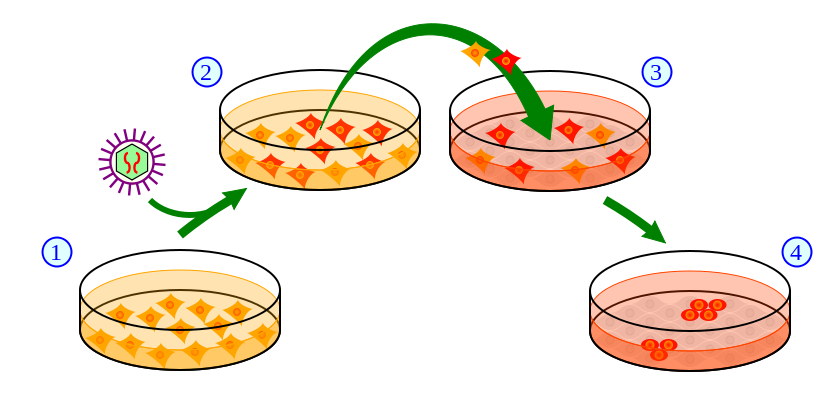
\includegraphics[width=0.7\textwidth]{../visualizations/ch4-methods/ipscprocess.png} 
	\caption[test.]{
		The four high-level steps taken to obtain iPSC cells \cite{img:ipscprocess}:
		(1) Grow a cell culture of donor cells, (2) transduce the genes associated with reprogramming into the cells via viral vectors, (3) isolate the cells expressing the transduced genes (in red) and culture them according to embryonic stem cell culture and, finally, (4) a small subset of the transfected cells become iPSC cells.
	}
	\label{fig:ipscprocess}
\end{figure}

HipSci provides a large repository of human induced pluripotent stem cell (iPSC) lines. iPSC cells are mature cells which have been reprogrammed to again become immature pluripotent (undetermined) cells. This process is visualized in Figure \ref{fig:ipscprocess}. As iPSC cell lines are not directly obtained from human donors, but rather from building a cell culture based on some initial donor cells, accessing raw RNA-seq reads is not constrained by the same data privacy regulations which prevented access to the raw RNA-seq reads from the GTEx project.


Concretely, over 300 cell lines from over 300 donors along with sequencing information based on RNA-seq is publicly available from the HipSci portal. From these we selected two different groups of cell lines:
\begin{itemize}
	
	\item the first group contains 25 biological replicates (that is, samples from different cell lines developed under the same conditions) of sensory neuron cell lines \cite{ipscneurons}. These cell lines were obtained by differentiating iPSC cells to sensory neuron cells.
	\item the second group contains 20 biological replicates of iPSC cell lines which weren't differentiated to any other cell type. Here care was taken to choose donors from whom at least two different iPSC cell lines were developed.
	
	%	iPSC cell lines: the second group of 20 biological replicates were taken from skin-tissue based iPSC cells which weren't differentiated to any other tissue. Here care was taken to choose donors from whom at least two different iPSC cell lines were developed. This allows us to test how well the learned features of the model generalize when applied to another library of the same tissue type from the same individual.
\end{itemize}

All used iPSC cells were originally obtained from skin cells. 

Selecting the samples in this way enables us to test cross-condition performance in three ways:
\begin{itemize}
	\item on the same cell type from the same donor, but from a different cell line. Here we expect the best generalization performance.
	\item on the same cell type, but a different donor.
	\item on a different cell type and from a different donor. Here we expect the worst generalization performance.
\end{itemize}


%From a biological perspective, it is interesting to see how splicing varies under different conditions. From a practical perspective, it is important to know how well the model generalizes when applied under different conditions. 
%This was the motivation to take cell lines from two different cell types. 
% For the analogue reason, the second group contained libraries of two different cell lines developed from the same donor of the same cell type. 
%of samples of we chose the samples from the second group so that we would have different at least one pair of samples from the 
%Cell-lines from two different tissue types were taken, as this will allows us to test how well 

The appendix contains the ENA Accession Numbers of the chosen samples in Section \ref{app:hipsci_celllines}.


%iPSC background probably here:
%some section about iPSC cells as relevant later on -- might skip all of this:
%The Nobel Prize in Physiology or Medicine of 2012 was awarded to Shinya Yamanaka and Sir John Gurdon "for the discovery that mature cells can be reprogrammed to become pluripotent". Pluripotent cells are cells which can differentiate into other cell types.
%process: take cell samples, then grow cell culture, make them pluripotent and use the pluripotent cells to differentiate into other ones
\section{Data processing}\label{sec:dataprocessing}
\subsection{Estimating PSI} \label{subsec:psiestimation}
%An often-used measure is to quantify alternative splicing is per cent spliced-in (PSI or $\Psi$).
%$\Psi$ is defined as the proportion of transcripts out of all transcripts that contain a given exon \cite{psi}. In other words, given a random transcript, it denotes the probability of a particular exon being included or excluded.
%Similarly, $\Psi_5$ is defined as the number of transcripts containing a particular alternative 3' splice site for a fixed 5' splice site. $\Psi_3$ is defined analogously as the number of transcripts containing a particular alternative 5' splice site for a fixed 3' splice site. $\Psi_5$ and $\Psi_3$ are particularly interesting to model the competition between different alternative splice sites.


%High-throughput sequencing of cDNA fragments (RNA-seq; Lister et al., 2008) has become a popular tool to investigate RNA expression and post-transcriptional regulation. Sequencing of the transcriptome reveals tens of thousands of transcripts expressed simultaneously (Mortazavi et al., 2008). Despite providing a deep and genome-wide view on post-transcriptional processing, current technologies cannot reveal transcripts in full-length due to limitations in read length.  [https://www.researchgate.net/publication/282645615_Alternative_Splicing_Signatures_in_RNA-seq_Data_Percent_Spliced_in_PSI/link/59e8404b458515c3630fe4e3/download]



%However, due to limitations in read length, they are not able to provide a full view of post-transcriptional processing so far.
%[majiq + berlin, https://elifesciences.org/articles/11752#abstract]
%'Despite constant technological advancement, the combination of limited coverage depth, experimental biases, and reads spanning only a small fraction of the variable parts of transcripts has left accurate mapping of transcriptome variations an open challenge (Alamancos et al., 2014).'
\subsubsection{Naive PSI estimation}\label{subsubsec:naivepsi}

Let \#IR be the number of reads giving evidence for a particular exon being included. Let \#ER be the numbers of reads giving evidence for a particular exon being excluded. A PSI value of 100\% indicates a constitutive exon which is always included, a score below 100\% includes an alternatively spliced exon. PSI can then be estimated as:
$$PSI = \frac{\#IR}{(\#IR+\#ER)}$$

Figure \ref{fig:psiestimation} illustrates the process of estimating PSI based on RNA-seq reads.  
The advantage of this estimate lies in its simplicity and flexibility. It is quick and easy to implement (hopefully bug-free). It is independent of library size. It can easily be adapted to estimate the PSI of a junction by redefining \#IR and \#ER to count the inclusion and exclusion read for that junction.

\begin{figure}[h]
	\centering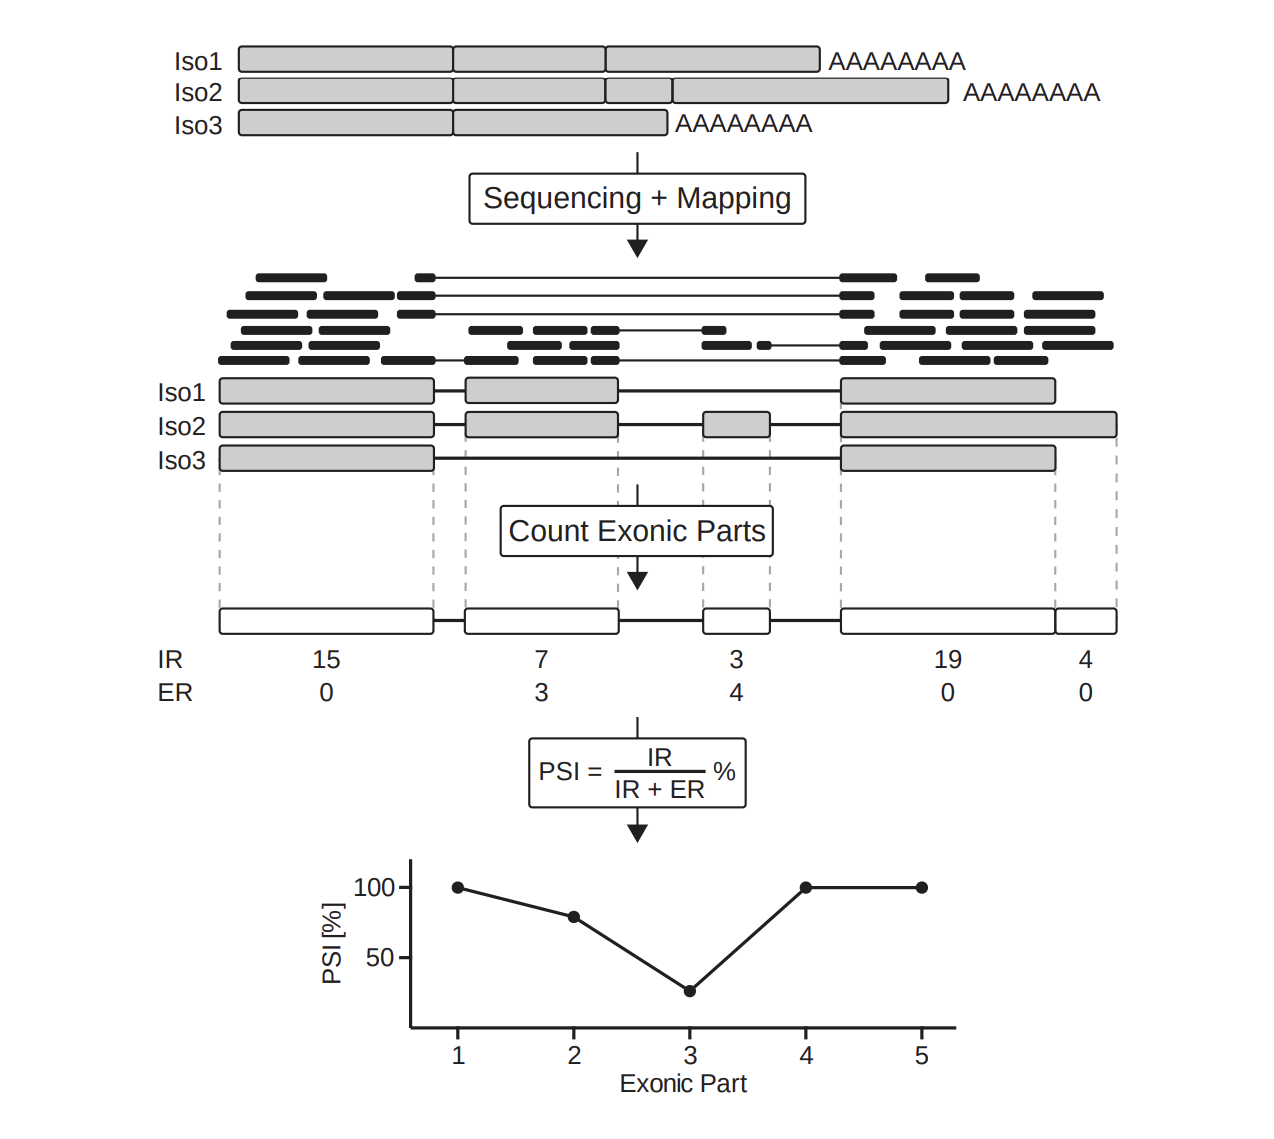
\includegraphics[width=0.8\textwidth]{../visualizations/ch4-methods/psi_estimation.png} 
	\caption{
		Process of estimating PSI based on RNA-seq reads \cite{berlinpsi}. First, the reads are mapped to the transcript. Based on annotation files, the reads overlapping exon/intron junctions are classified as including or excluding reads for a particular exon. Based on the observed IR and ER, the PSI for a given exon is then estimated.
	}
	\label{fig:psiestimation}
\end{figure}
%lix says make sure this figure precedes list below; added [h]
%'deceptively simple'?

However, this estimate also has various issues:
\begin{enumerate}[label=(\alph*)]
	\item It doesn't account for uncertainty. A rarely expressed gene may only experience a few reads of a particular exon leading to a very uncertain estimate. If we observe 1 IR and 1 ER for exon E1, and 15 IR and 15 ER for exon E2, then the estimated PSI of both exons is 50\%.
%	: $PSI_{E1} = \frac{1}{2} = 50\%$. Compare this to E2 where we observed 15 inclusion and 15 exclusion reads: $PSI_{E2} = \frac{15}{30} = 50\%$.\\
	The estimate of $PSI_{E2}$ is likely to be more accurate, but this information is not contained in the estimate. Concretely, these two samples would be treated as equally important by the network even though they likely shouldn't.
	
	To account for this, it is possible to only count exons who experienced at least a certain number of reads. However, raw read counts are unreliable when not accounting for overall gene expression: 10 reads in a lowly expressed gene may be as significant as 20 reads in a highly expressed gene. There are several measures for the abundance of a gene: Reads Per Kilobase Million (RPKM), Fragments Per Kilobase Million (FPKM) and Transcripts Per Kilobase Million (TPM). Of these, TPM is usually the most common choice. Therefore, a better solution is likely to only count reads from genes whose TPM is above a certain threshold. \\
	Note that there is not a principled way to choose this threshold. The choice between a threshold which e.g. filters 5\% or 20\% of the samples is a trade-off between data quality and data quantity. In practice, the `optimal' cutoff threshold will be unknown and vary from dataset to dataset.
	% reformulate once again to say just take TPM values bitch no cut-off
	%	However, assuming this solution is taken, there are an additional two aspects worth discussing:
	%	However, Assuming that one obtains a read count normalized by the gene expressiveness, there are two further aspects worth discussing:
	%	\begin{enumerate}
	%		\item 
	%		\item There is not a principled way to choose the cutoff threshold. The choice between a threshold which e.g. filters 5\% or 20\% of the samples is a trade-off between data quality and training samples. In practice, the optimal way to choose the cutoff threshold will be unknown and vary from dataset to dataset.
	%	\end{enumerate}
	% https://www.rna-seqblog.com/rpkm-fpkm-and-tpm-clearly-explained/
	
	
	\item Reads aligning purely to the flanking constitutive exons are ignored. While these reads could have occurred in transcript isoforms containing or excluding the cassette exon, they still provide latent evidence. % for whether the cassette exon was included or not. 
	In isoforms where the cassette exon is included, the total length of the isoform is longer which means that reads are distributed over a larger area. This leads to a comparatively reduced proportion of reads across the flanking exons when the exon was included and vice versa. The estimate neglects to take this information into account.
	%	This estimate ignores reads that align to the bodies of the flanking constitutive exons, which could have derived from either isoform. Nevertheless, these constitutive reads contain latent information about the splicing of the alternative exon, as higher expression of the exclusion isoform will generally increase the density of reads in the flanking exons relative to the alternative exon, and lower expression of the exclusion isoform will decrease this ratio of densities.
	%	[MISO]
	%	This is the reason why I wanted access to raw RNA-seq reads
	\item Related to (a), typically multiple samples or biological replicates of a given experiment are available. It is desirable that reads across multiple samples can be integrated to give a more well-adjusted estimate. How to best achieve this is not obvious. Read depths between multiple libraries may vary and this should be accounted for. 
	%[possible other issues here and then make this another itemization]
	\item IRs and ERs must be normalized for exon length to obtain meaningful results. For a long exon, the majority of reads will be IRs because they can be located over a much larger area than the ERs who must overlap with the 0-length feature of the splicing junction (see Figure \ref{fig:readlengthnorm}). This can be accounted for by normalizing for the possible number of start positions of each read population \cite{berlinpsi}:
	$$\#IR_{norm} = \frac{\#IR}{exon\_length + read\_length -1}$$
	$$\#ER_{norm} = \frac{\#ER}{read\_length - 1}$$
	% included berlin graphic as favouring action over inaction and well I don't think (I hope) I have an excessive amount of graphics yet
	%	Note that this assumes that reads are uniformly distributed across a transcript isoform. It is well-known that RNA-seq reads are biased .... [get paper from Liz/Wilfred]
	
	%	thought: this normalization doesn't obviously seem correct to me on second thought. an ER can be found at two junctions, so that would double the number of possible read starts
	%	IR can only start from position 0 to exon.length-read.length of the exon can't they?
	%	won't do anything about this but will want to use weaker claim
	%	I think you can't really do normalization for junction counting
	
	%	The goal of these adjustments is not to arrive at perfect estimates, but rather to alleviate the influence of systematic biases as much as possible. 
	
	%: could add that even then reads across a gene aren't evenly distributed
	% See https://bmcbioinformatics.biomedcentral.com/articles/10.1186/1471-2105-12-290
	
	\item Reads may be misattributed. The motivation for analyzing splicing at a level of alternative splicing events is that full gene isoforms can not reliably be quantified given the currently available short RNA-seq read lengths. However, this issue may still occur at the splicing event level when two splicing variants of an exon share a junction. This is illustrated in Figure \ref{fig:misattribution}.
	This misattribution of a read can only be corrected by considering circumstantial evidence, similar to (b); for instance, read counts on the non-shared junction may give evidence regarding which splicing event the read at the shared junction belongs to.
\end{enumerate}


\begin{figure}
	\centering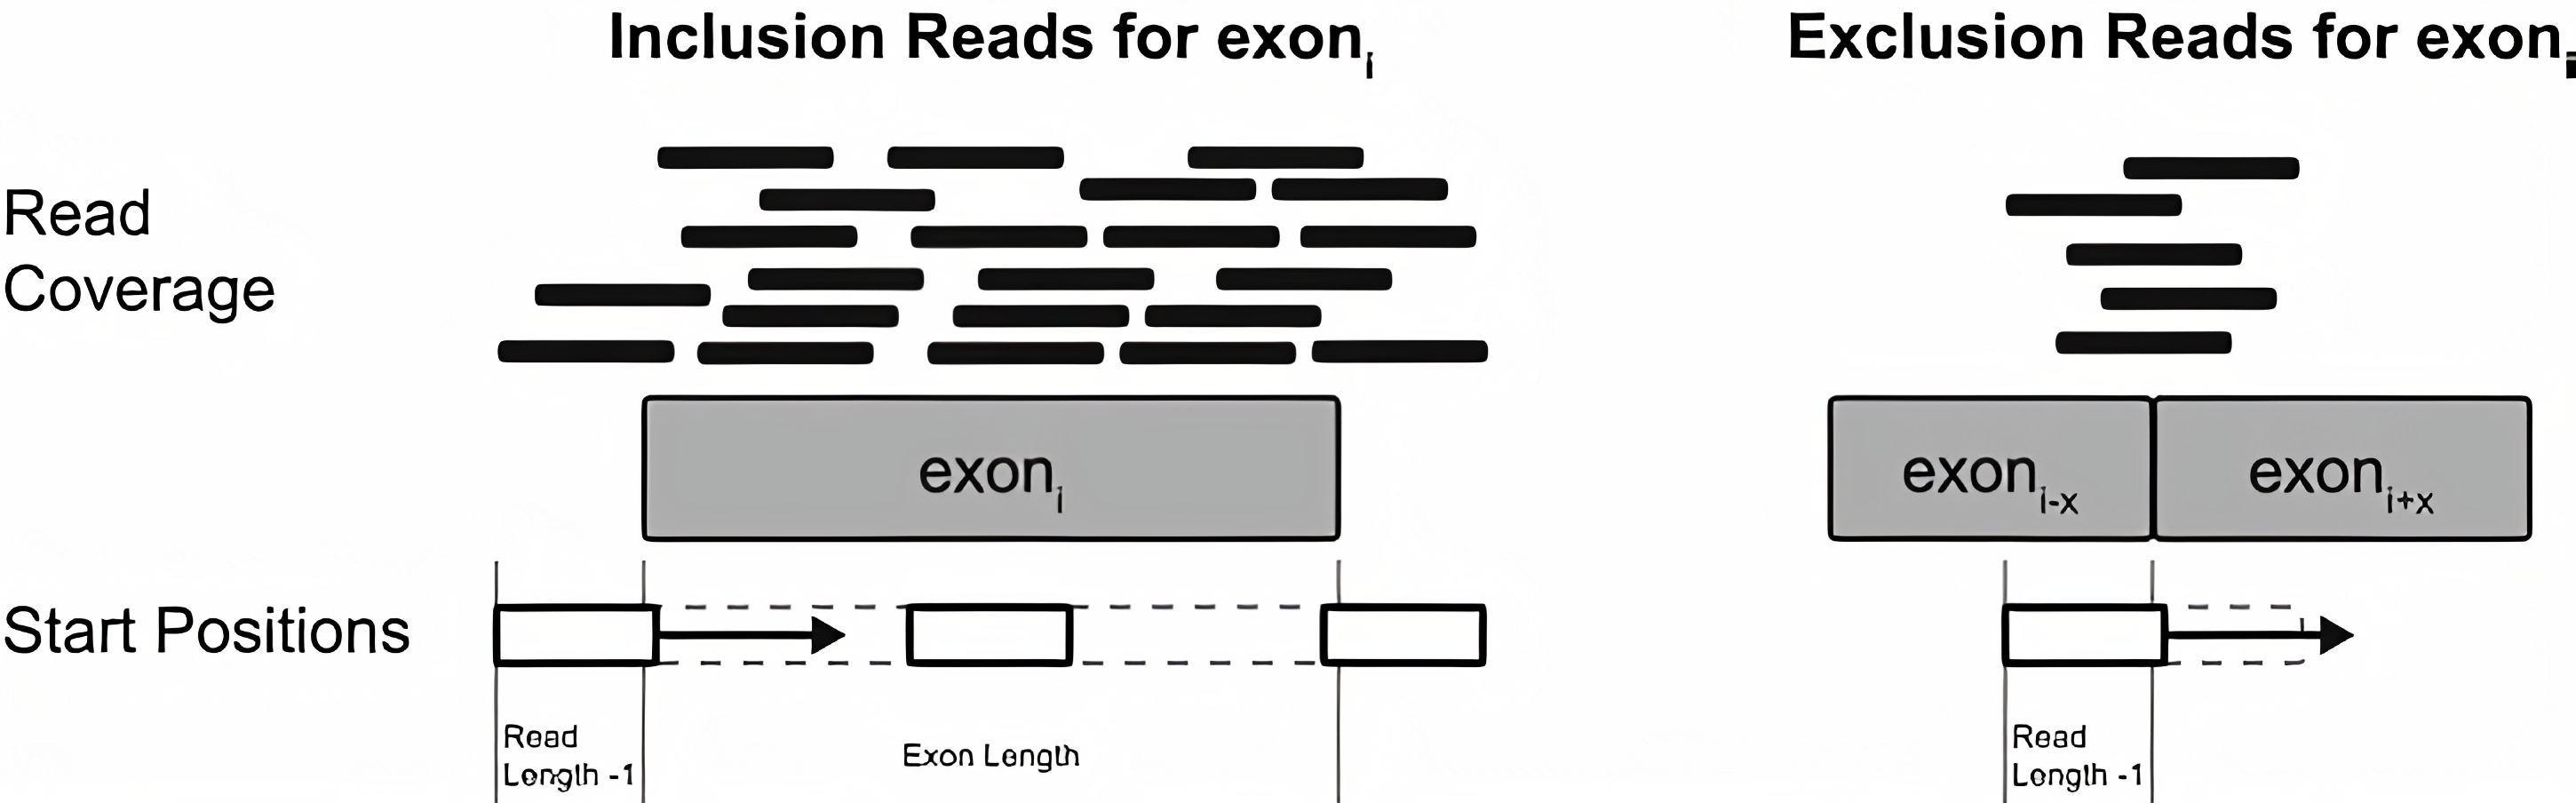
\includegraphics[width=0.85\textwidth]{../visualizations/ch4-methods/read_length_normalization.jpg} 
	\caption{
		The need for read length normalization when estimating PSI \cite{berlinpsi}. An IR (left) can be located anywhere over the exon and around the junction. An ER (right) can only be located where it crosses the exon-exon junction. Thus, any PSI estimation which does not account for this will be biased towards estimating higher PSI values than accurate. 
	}
	\label{fig:readlengthnorm}
\end{figure}

\begin{figure}
	\centering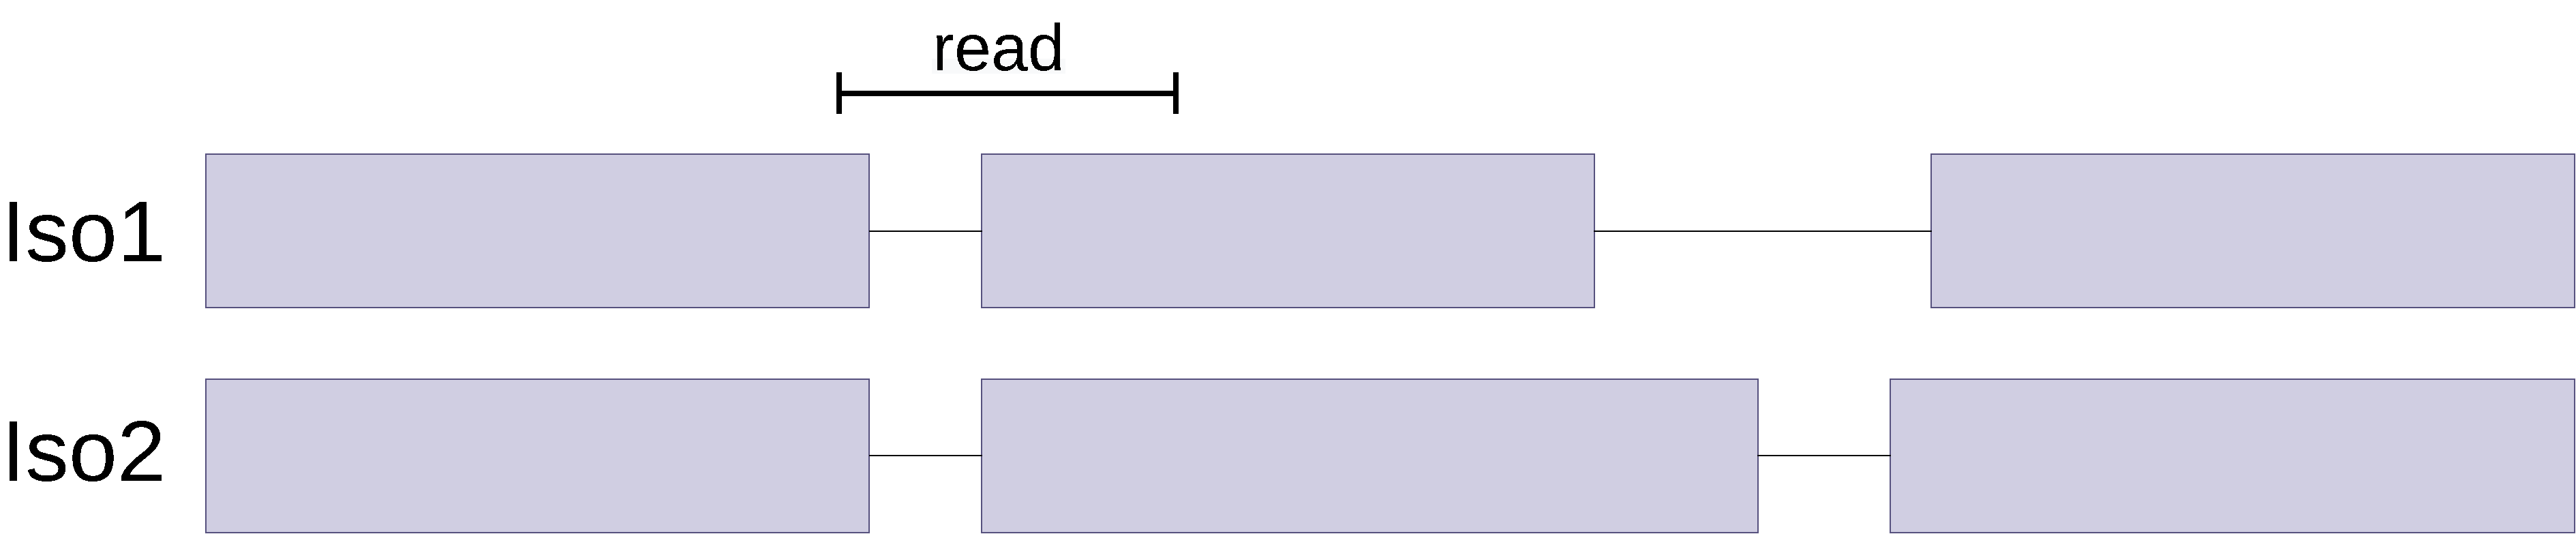
\includegraphics[width=0.7\textwidth]{../visualizations/ch4-methods/visualizations-misattribution.pdf} 
	\caption{The read across the exon-exon junction may be attributed to isoform 1 or isoform 2. Consequently, it may also be attributed to the first or second splicing variant of the middle exon.}
	\label{fig:misattribution}
\end{figure}

%hopefully was able to demonstrate that this estimate is problematic and may easily be unreliable.
%Due to these issues relating to calibrating for uncertainty, to not making use of all of the available evidence, to integrating reads across multiple samples and misattributing reads, is estimate is problematic.
Any estimate of PSI that doesn't account for all, or at least the majority of these issues, will likely be very unreliable. 

\subsubsection{A word of caution} \label{subsubsec:caution}
However, even if all of these issues are addressed optimally, the resulting PSI estimate would still be imperfect. For instance, the `solutions' for (a) and (d) implicitly rely on the assumption that reads across a transcript are evenly distributed. It is well-known that sequence reads across a transcript aren't equally distributed due to biases relating to GC-content \cite{gccontentbias}, gene length and dinucleotide frequencies \cite{rnaseqbiascorrection}.
% or transcript length bias. 
% there is also transcript length bias, see https://biologydirect.biomedcentral.com/articles/10.1186/1745-6150-4-14
% but this bias is more about biases between transcripts rather than within a given transcript
%[ list of biases duplicate reads, stacking reads]. 
%: stashed for now; https://bmcbioinformatics.biomedcentral.com/articles/10.1186/1471-2105-12-290
% https://www.the-scientist.com/news-opinion/technical-bias-widespread-in-rna-seq-datasets-66766#:~:text=Love%20adds%20that%20there%20are,length%2Drelated%20biases%20as%20well.
% https://emea.support.illumina.com/bulletins/2017/04/considerations-for-rna-seq-read-length-and-coverage-.html#:~:text=Experiments%20looking%20for%20a%20more,for%20mRNA%2Fwhole%20transcriptome%20sequencing.
%https://genomebiology.biomedcentral.com/articles/10.1186/s13059-016-0881-8
These biases are not easily quantifiable and can never be perfectly corrected for. Thus, the PSI estimate will always be affected by these biases. 

%and even already adjusted read estimates (e.g. for gene expressiveness) are still biased. \\
In more general terms, the data on which the estimate is based on is biased in multiple complex, dynamically interacting ways and this will always lead to downstream effects independent of the preprocessing method used. The question is not whether the resulting estimate is still biased, but rather if the effect of systematic biases influencing it can be alleviated enough for the estimate to be useful. In this study, we answer this question in an empirical way by testing datasets resulting from four different PSI estimation methods. We now introduce the exact datasets we use and which PSI estimation method was used to obtain them. 
%i basically says here that unbiasing rna-seq data will never be possible - opinions from wil and liz? lol
\subsubsection{Dataset based on HEXEvent}
% https://www.ncbi.nlm.nih.gov/pmc/articles/PMC1431573/
The HEXEvent database provides EST count-based PSI estimates for exons and facilitates standard filtering steps (e.g. only select cassette exons). 
The baseline paper \cite{dsc} takes HEXEvent as starting point and generates three different datasets respectively only containing cassette exons, exons with an alternative 3' splice and exons with an alternative 5' splice site. Each of these datasets also contains constitutive exons. To account for the biases inherent in EST data, it applies multiple filtering steps such as requiring a minimum number of supporting ESTs and only using exons which display a single type of alternative splicing. They make the resulting datasets publicly available and we use the dataset containing cassette exons for direct comparability. 

However, it should be noted that HEXEvent uses the criticized naive estimation method for PSI, i.e., they estimate PSI as $PSI = \frac{\#IR}{(\#IR+\#ER)}$. Except for requiring a minimum number of supporting ESTs, none of the five main critique points from \ref{subsubsec:naivepsi} are explicitly accounted for by \cite{dsc}. The EST data available from UCSC is based on many different tissues which may lead to the derived alternative splicing behaviour being an average of the splicing behaviour of many tissues which never occurs in any singular tissue. %distort view, confuse nice words here
Therefore, care should be taken when drawing conclusions based on the PSI estimates of this dataset. 

\subsubsection{Our PSI estimation implementation} \label{subsubsec:implementedpsiestimation}
To obtain a PSI estimate based on the publicly accessible exon-exon junction read counts of the GTEx project, we implement our own PSI estimation method. We are not able to use the PSI estimation methods from the literature we introduce below, as they require access to the raw RNA-seq reads which we don't have access to due to data privacy regulations.

GTEx publicly gives access to anonymized information about which sample types were taken from which donor. We use this information to find a donor from whom brain cortex tissue, cerebellum tissue and heart tissue samples were taken. For each tissue sample, we derive two datasets: one exon-centric dataset in which we estimate PSI for cassette exons and one intron-centric dataset in which we estimate PSI for junctions. 
% would give more details about how cassette exons/junctions are selected in the respective datasets here
We obtain six datasets in total.

Fundamentally, our PSI estimation relies on the formula $PSI = \frac{\#IR}{(\#IR+\#ER)}$. However, before computing PSI, we also apply the following filtering and normalization steps:
\begin{itemize}
	\item Cassette exons which are shorter than 25 nt and introns which are shorter than 80 nt are excluded. Exons and introns of these lengths constitute less than 1\% of exons and introns in the genome and are usually an artefact of sequencing errors \cite{dsc} \cite{shortintrons}.
	\item GTEx provides access to TPM values for each gene from a sample. Addressing point (a) from \ref{subsubsec:naivepsi}, we obtain the TPM-adjusted read counts via $\#IR^{TPM} = \frac{\#IR}{TPM}$ and $\#ER^{TPM} = \frac{\#ER}{TPM}$. To address spurious reads from lowly-transcribed genes having a disproportionate impact, we only count reads from genes whose TPM is larger than 10. This filters around 84\% of genes which in turn filters around 56\% of the junctions. This is the most stringent filtering step we apply. 
	
	%	This is by far the most stringent filtering method we apply, leading to about two-thirds of genes being filtered. This cut-off was chosen so aggressively as data quality is paramount. More details are given in Figure %\ref{fig:tpm_distribution}.
	\item Adressing point (d) about IRs naturally being more common than ER, we estimate the read length of the RNA-seq reads to be 150 on average \cite{gtex_read_length} and apply the proposed normalization method: $\#IR^{TPM}_{norm} = \frac{\#IR^{TPM}}{(exon length + 149)}$ and $\#ER^{TPM}_{norm} = \frac{\#ER^{TPM}}{149}$.
\end{itemize}

Using the normalized \#IR and \#ER of all exons and junctions remaining after filtering, we then compute PSI: $PSI = \frac{\#IR^{TPM}_{norm}}{(\#IR^{TPM}_{norm}+\#ER^{TPM}_{norm})}$. 

Comparing our estimation method to the standards set out by \ref{subsubsec:naivepsi}, this estimate fails to take into account the information contained in non-junction reads, as we simply don't have access to them.
This estimate also does not aggregate the information from multiple biological samples, although we took care to choose the donor with tissue samples from brain cortex, cerebellum and heart, whose total read count was the highest. 
Reads may also be misattributed in our cassette exon PSI estimation as described in (e). Note that misattribution is not an issue when estimating the PSI of junctions.
%The initial dataset contained roughly 10 million total exon-exon junction read count for each tissue distributed over roughly 330,000 unique junctions. More statistics about this dataset, and the others, are given in Section \ref{subsec:datasetstatistics}. 

%After the PSI values have been obtained as described above, we apply the final sample processing steps as described in \ref{subsec:finalsampleprocessing}.
% tpm value histogram
%\begin{figure}
%	\centering%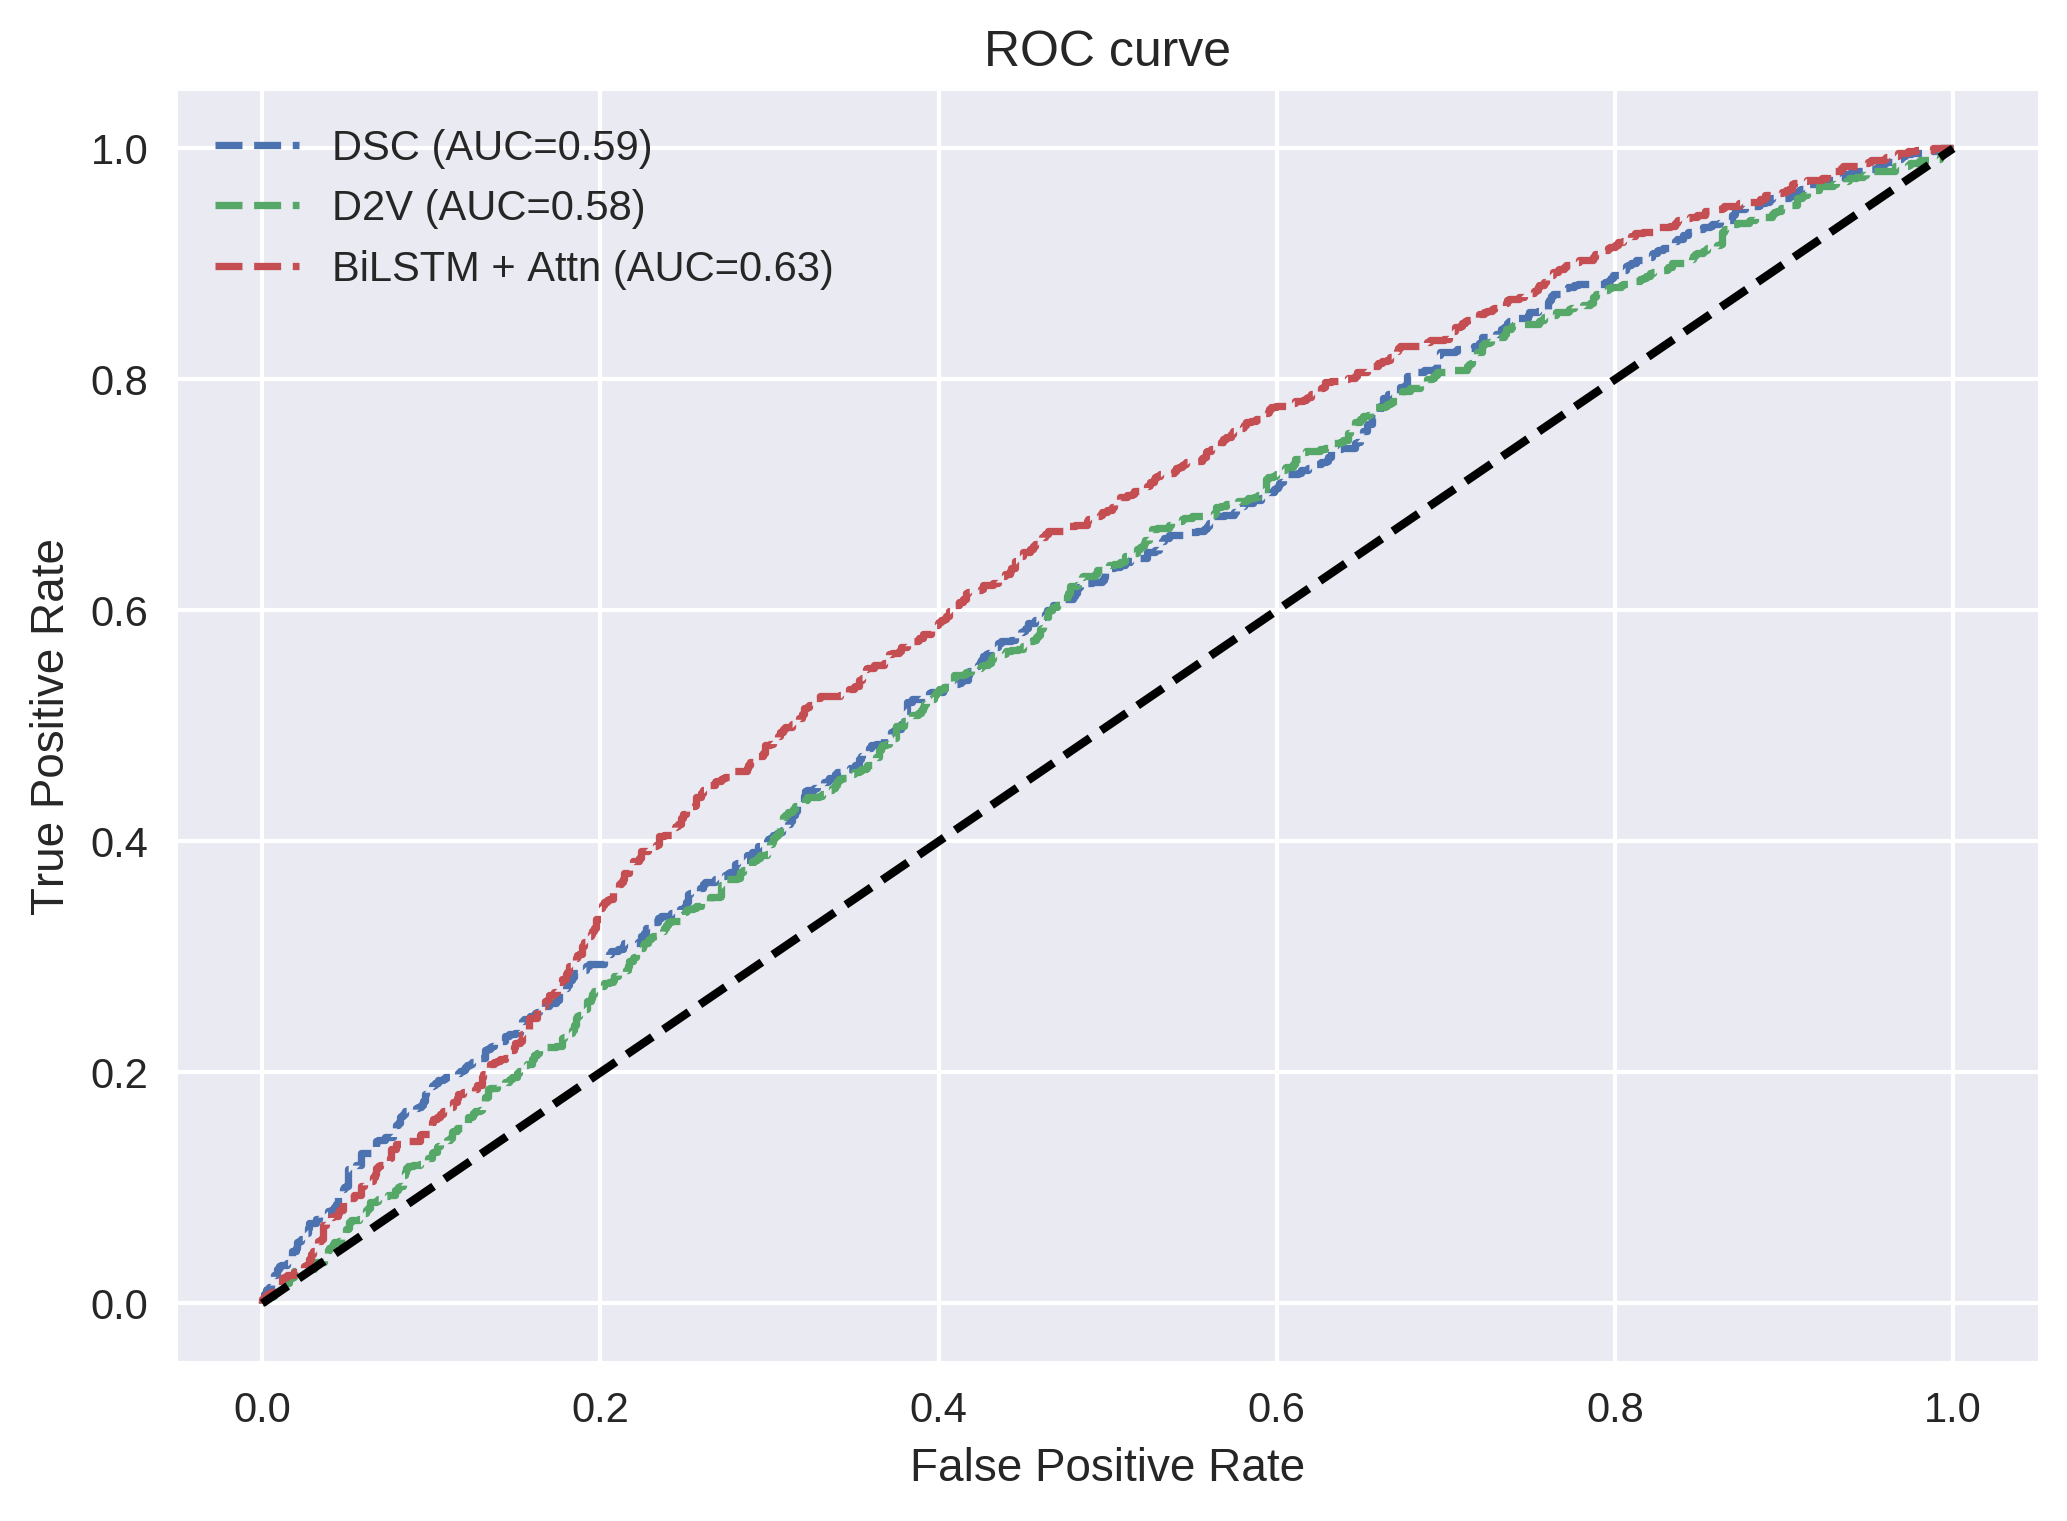
\includegraphics[width=0.7\textwidth]{../visualizations/suppa_cross_model_roc_auc_comparison.png} 
%	\caption{
%		Distribution of TPM values. The cut-off we chose is marked in red. Concretely, this leads to filtering ... out of ... genes. }
%	\label{fig:tpm_distribution}
%\end{figure}
%1) TPM: Only take reads from genes across a certain TPM into account (because random spurious reads from low TPM genes could have an outsized effect on the estimation). Say that your weight reads according to the respective TPM. Show TPM distribution and say what TPM threshold you use.\\
%2) Latent information: Say how there is nothing you can do, due to only having access to the junction reads themselves. \\
%3) Multiple samples: Unclear how to best do this and skipped for now. However, basing estimation based on the sample with the maximum total amount of reads. \\
%4) Start pos normalization: Say that you estimate read length to be 150 and do this. \\
%  mention junction datasets
% potentially even more details; eg how you use this heuristic of checking the 10 samples past the current one
%  add details such as exact name of individuals used and 




\subsubsection{More sophisticated PSI estimation approaches}

Several approaches have been developed which try to address the issues in estimating PSI. However, many of these focus purely on the differential splicing changes between conditions (in the form of $\Delta$ PSI) and don't directly report the PSI in a given condition which is what we are initially interested in. Of the methods directly reporting PSI, we chose two fast methods which represent different approaches to PSI estimation: SUPPA and MAJIQ. SUPPA is primarily based on quantification of transcripts, while MAJIQ is based on building up a splicing graph. MAJIQ has already been used for the construction of similar datasets before \cite{jha}.
%\ref{fig:dataset_creation_process} shows the high-level steps taken when using SUPPA and MAJIQ to create datasets for training.


% inaccurate as I don't think SUPPA directly takes BAM / kinda unnessessary either way
%\begin{figure}
%	\centering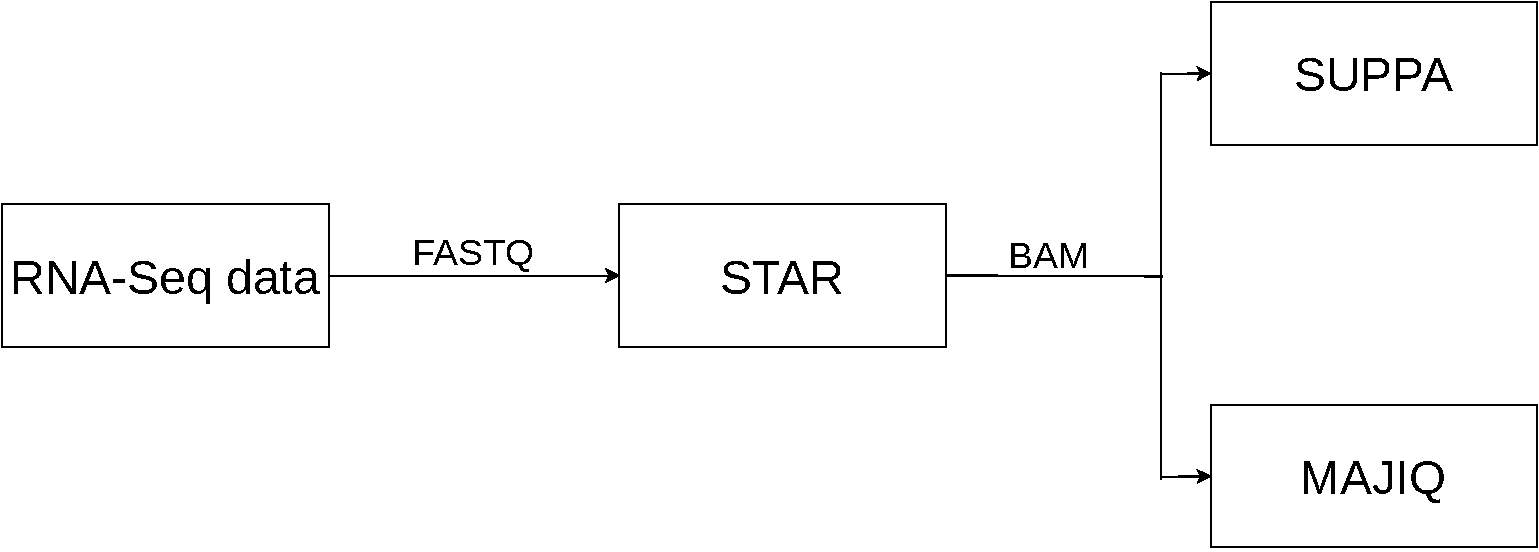
\includegraphics[width=0.7\textwidth]{figures/d2v-Page-3.pdf} 
%	\caption{Data flow when using MAJIQ or SUPPA to create a training dataset. }
%	\label{fig:dataset_creation_process}
%\end{figure}
%isoform-based vs count-based methods
%	count-based methods = exon based and event-based methods
\subsubsection{SUPPA}\label{subsubsec:suppa}
SUPPA \cite{suppa2} estimates the PSI value for each alternative splicing event based on transcript abundance. It operates in 2 steps for quantifying the PSI of an alternative splicing event:
\begin{itemize}
	\item Given an input annotation file in GTF format, it generates the transcript isoforms which count as IR or ER for a given alternative splicing event.
	\item Given the information which transcript count as IR or ER from 1) and how frequently each transcript occurs, it estimates the PSI value via $PSI = \frac{TPM_{IR}}{TPM_{IR} + TPM_{ER}}$. $TPM_{IR}$ and $TPM_{ER}$ respectively refer to the total TPM of transcripts supporting a certain exon being included or excluded. 
\end{itemize}
SUPPA can integrate the TPM values from multiple samples.
%because it is so naive is probably the reason why it performs so badly
%!perhaps add steps 1/2/3 to this graphic?


\textbf{Using SUPPA:}
SUPPA requires a GTF annotation file and a file quantifying the abundance of each transcript. A GENCODE version 34 annotation file obtained from Ensembl was used as an annotation file. Salmon \cite{salmon} was used to quantify the relative abundance of each transcript in TPM. Salmon's quantification is based on the raw RNA-seq reads in FASTQ format, takes into account experimental attributes and corrects for biases commonly observed in RNA-seq data. After extracting the TPM values provided by Salmon into the format required by SUPPA (a tsv-file with one column for the transcript id and one column for the TPM value), SUPPA estimates the PSI for each alternative splicing event.
%[https://github.com/comprna/SUPPA/releases/tag/v2.3 if I feel like it]

%SUPPA operates on at a transcript level and therefore implicitly relies on the assumption that all transcripts of a given gene are known - this is often not the case. Of the discussed issues in \ref{subsubsec:naivepsi}, it only accounts for 2 of them: 
SUPPA's main competitive advantage for PSI estimation lies in its speed and low memory overhead compared to other methods \cite{suppa} (which it achieves through leveraging fast transcript quantification methods such as Salmon), not necessarily that it achieves the best accuracy. This becomes apparent when judging how well SUPPA addresses the issues we laid out in \ref{subsubsec:naivepsi}: of these addresses it only (c) - the integration of evidence from multiple samples. SUPPA focuses exclusively on alternatively spliced exons and thus we are not able to derive a list of constitutive exons from SUPPA. Since SUPPA operates at the transcript level, it implicitly relies on the assumption that all transcripts of a given gene are known - this is often not the case. Therefore, it remains to be seen whether the estimation of SUPPA is accurate enough for our purposes.


% this was taken from the results section
%in retrospect, SUPPA was not the best choice for dataset processing. It operates at a transcript level and therefore implicitly relies on the assumption that all transcripts of a given gene are known - this is often not the case. Additionally, it does not make it possible to generate a list of non-cassette constitutive exons, therefore roughly halving the size of the training set and the number of samples the model can learn from. Its PSI estimation is very simplistic and doesn't account for multiple of the issues highlighted in \ref{subsec:psiestimation}. 



\subsubsection{MAJIQ}\label{subsubsec:majiq}
Modeling Alternative Junction Inclusion Quantification (MAJIQ) builds up a splice graph \cite{majiq2} which contains exon as vertices and junctions as edges. An edge is added between two vertices if a transcript isoform is found in which they share a junction (that is if the exons are neighbours and everything between them has been spliced out).
Constitutive exons are vertices with two incoming edges.
Vertices which have more than 3 incoming edges are denoted as local splicing variations (LSV). This problem formulation allows MAJIQ to model more complex splicing events (rather than the ones from \ref{fig:altsplicingforms}), although we won't leverage this extra capability here. Figure \ref{fig:splice_graph} shows an example splice graph. Importantly, apart from estimating $\Delta$ PSI between different conditions, MAJIQ is also able to directly estimate PSI for a given condition. The estimation is done using a combination of read rate modelling, Bayesian PSI modelling and bootstrapping. The only issue from \ref{subsubsec:naivepsi} MAJIQ doesn't account for is (b): the integration of the information from non-junction reads. Thus, we expect MAJIQ's PSI estimates to be the most accurate of all methods we are testing.
% looked at mjiq paper; it only seems to look at juntons
% hadnles eg point 5. by only looking at junctions until the very end and modelling eg cassette exons as two distinct LSVs --- ie each junction will have its own PSI


\begin{figure}
	\centering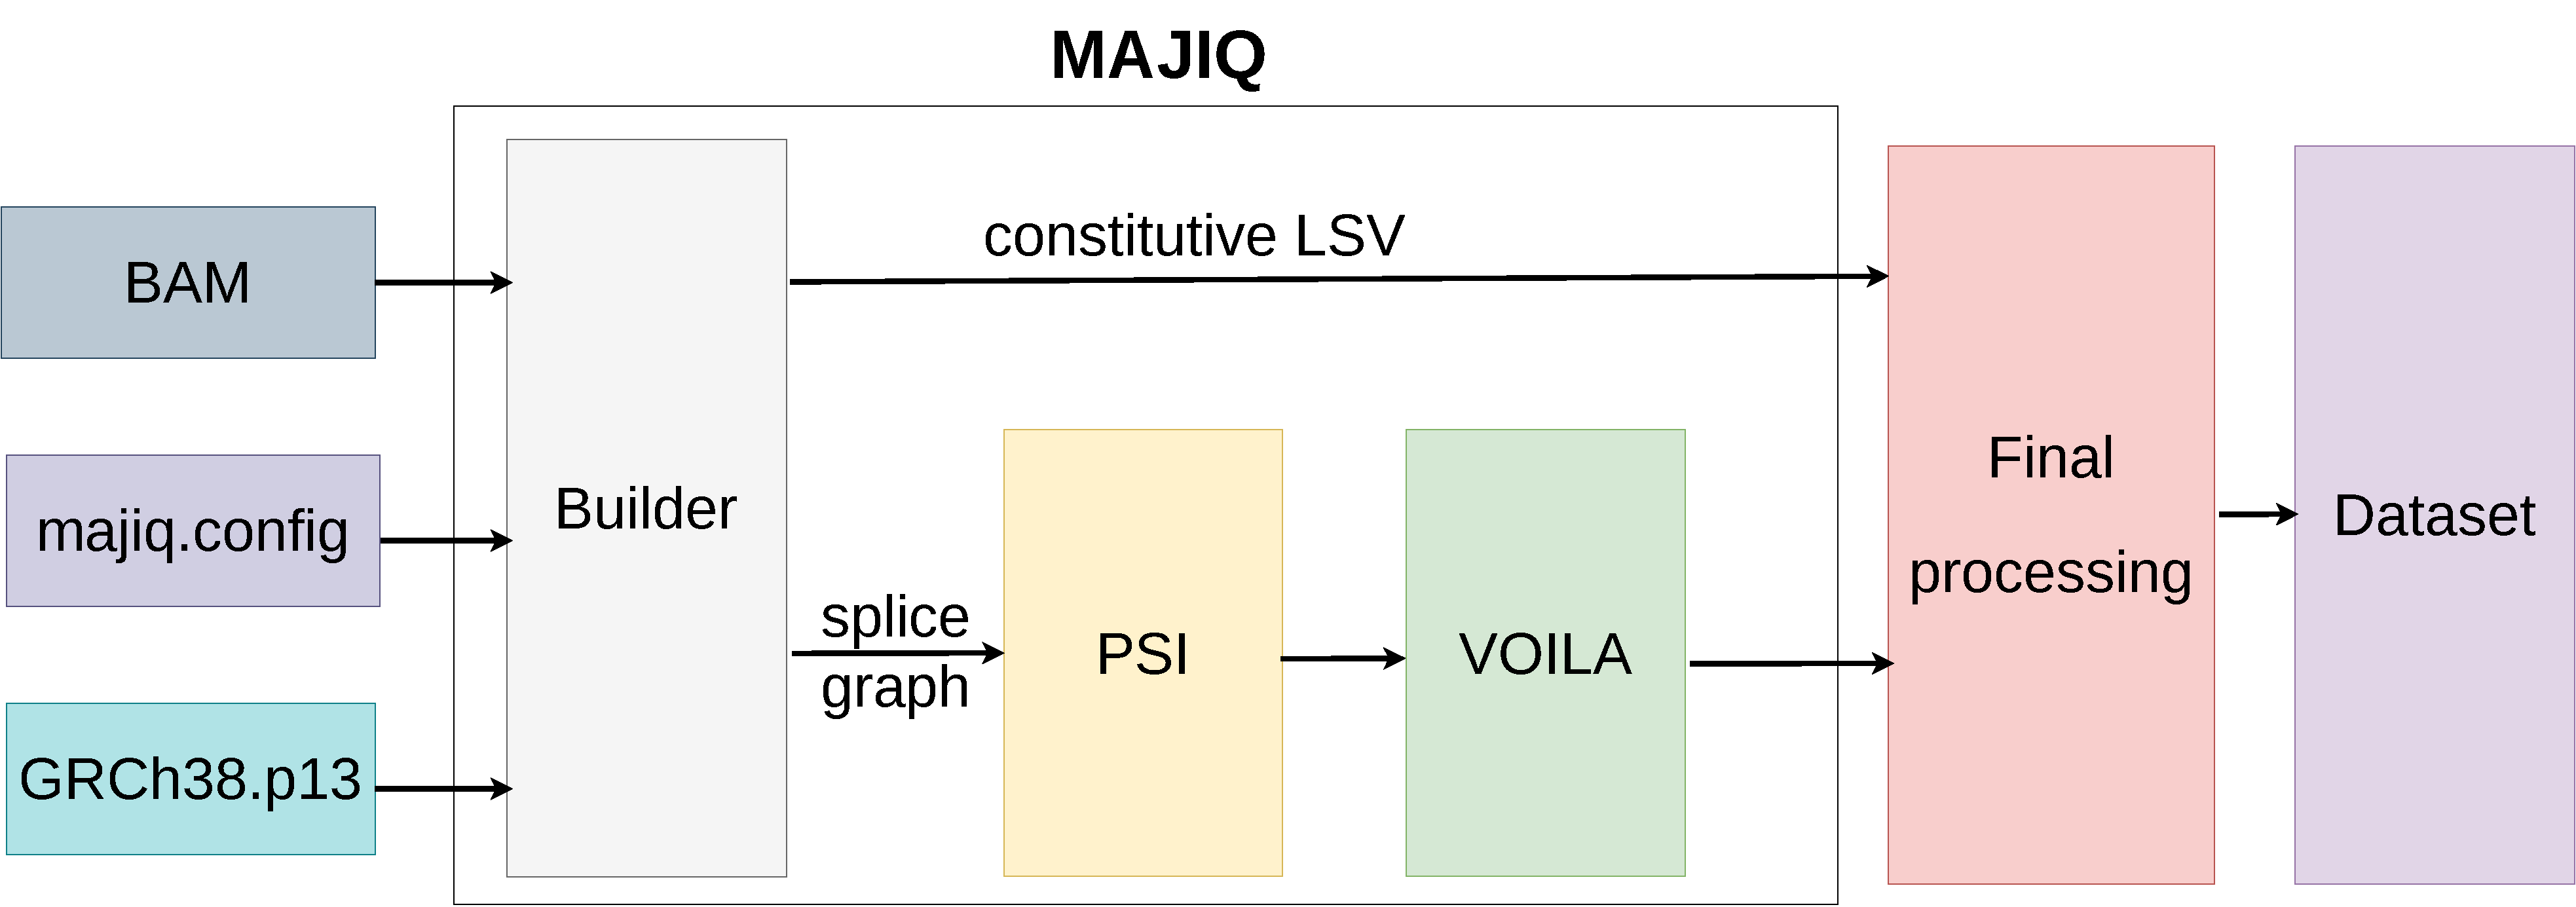
\includegraphics[width=0.85\textwidth]{../visualizations/ch4-methods/visualizations-majiq.pdf} 
	\caption{Data flow when using MAJIQ to create a training dataset. }
	\label{fig:majiq_dataset_creation_process}
\end{figure}

\begin{figure}
	\centering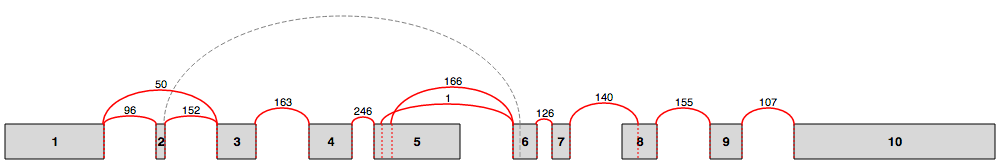
\includegraphics[width=1\textwidth]{../visualizations/ch4-methods/splice_graph.png} 
	\caption{An example splice graph as displayed in VOILA \cite{majiq2}. Exons, represented by grey rectangles, are connected with another exon via an edge, if a junction between the exons (or a variant of them) is observed. The number above an edge displays the number of observed raw reads spanning a particular exon-exon junction.}
	\label{fig:splice_graph}
\end{figure}

\textbf{Using MAJIQ:} MAJIQ requires sequence files in bam format (along with their respective index files) and an annotation DB (we used human GRCh38 release 13) in gff3 format. The bam format is a format for aligned RNA-seq reads. 
To this end, the raw reads from each sample were uploaded to the bioinformatics data processing platform Galaxy \cite{galaxy} from the European Nucleotide Archive (ENA). For each sample, the raw reads in FASTQ format were then mapped to the reference genome GRCh38 \cite{hg38} using STAR \cite{star}. STAR produces the required bam and bai format files as output.

MAJIQ use then proceeds in three stages. First MAJIQ Builder takes a configuration file, the gff3 annotation and the bam and bai files of all samples as input and builds up the splicing graph. At this stage, MAJIQ also identifies constitutive exons and optionally saves them to a file. This option was used.
Secondly, MAJIQ PSI estimates the PSI of the LSV candidates obtained through MAJIQ Builder. MAJIQ PSI improves the accuracy of its PSI estimate by integrating evidence across multiple samples.
Finally, the obtained LSVs can be visualized using VOILA. See Figure \ref{fig:voilaexample} for an example output of VOILA. VOILA also allows filtering of LSV according to type and we used this to obtain the estimated PSI values of all exon skipping LSVs. The filtered LSV along with the constitutive exons obtained from MAJIQ Builder were then used for processing as described in Section \ref{subsec:finalsampleprocessing}.\\
%The latest version of MAJIQ available as of July 2020 was used (MAJIQ v2.0).


\begin{figure}
	\centering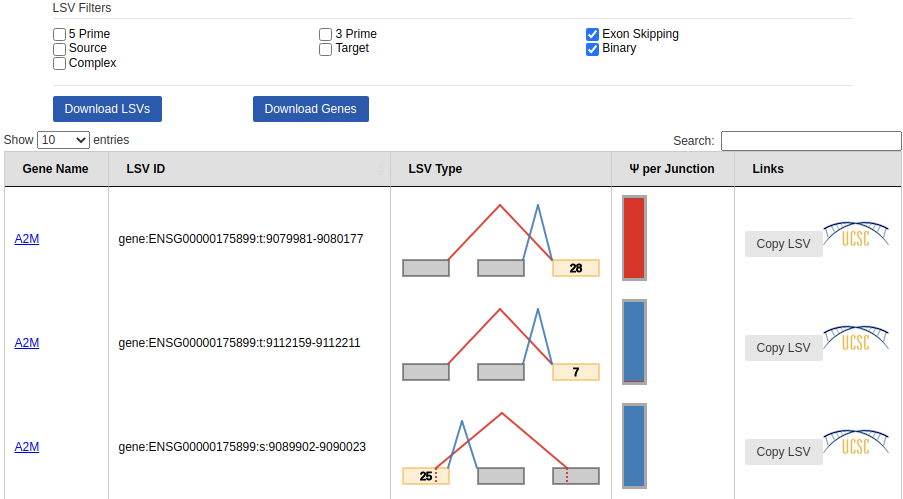
\includegraphics[width=0.85\textwidth]{../visualizations/ch4-methods/voila_example.png} 
	\caption[Four-chamber illustration of the human heart.]{Example output of VOILA while filtering for LSV which only experience exon skipping and no other alternative splicing event. }
	\label{fig:voilaexample}
\end{figure}


Our implementation of PSI estimation was applied to the GTEx dataset. SUPPA and MAJIQ were applied to the data from the HipSci repository. We refer to the GTEx-based and with our own PSI estimation method processed dataset, to the HipSci-based and with SUPPA processed dataset and to the HipSci-based and with MAJIQ processed dataset as GTEx dataset, HipSci SUPPA dataset and HipSci MAJIQ dataset for brevity. 
\subsection{Final sample processing} \label{subsec:finalsampleprocessing}

\begin{figure}
	\centering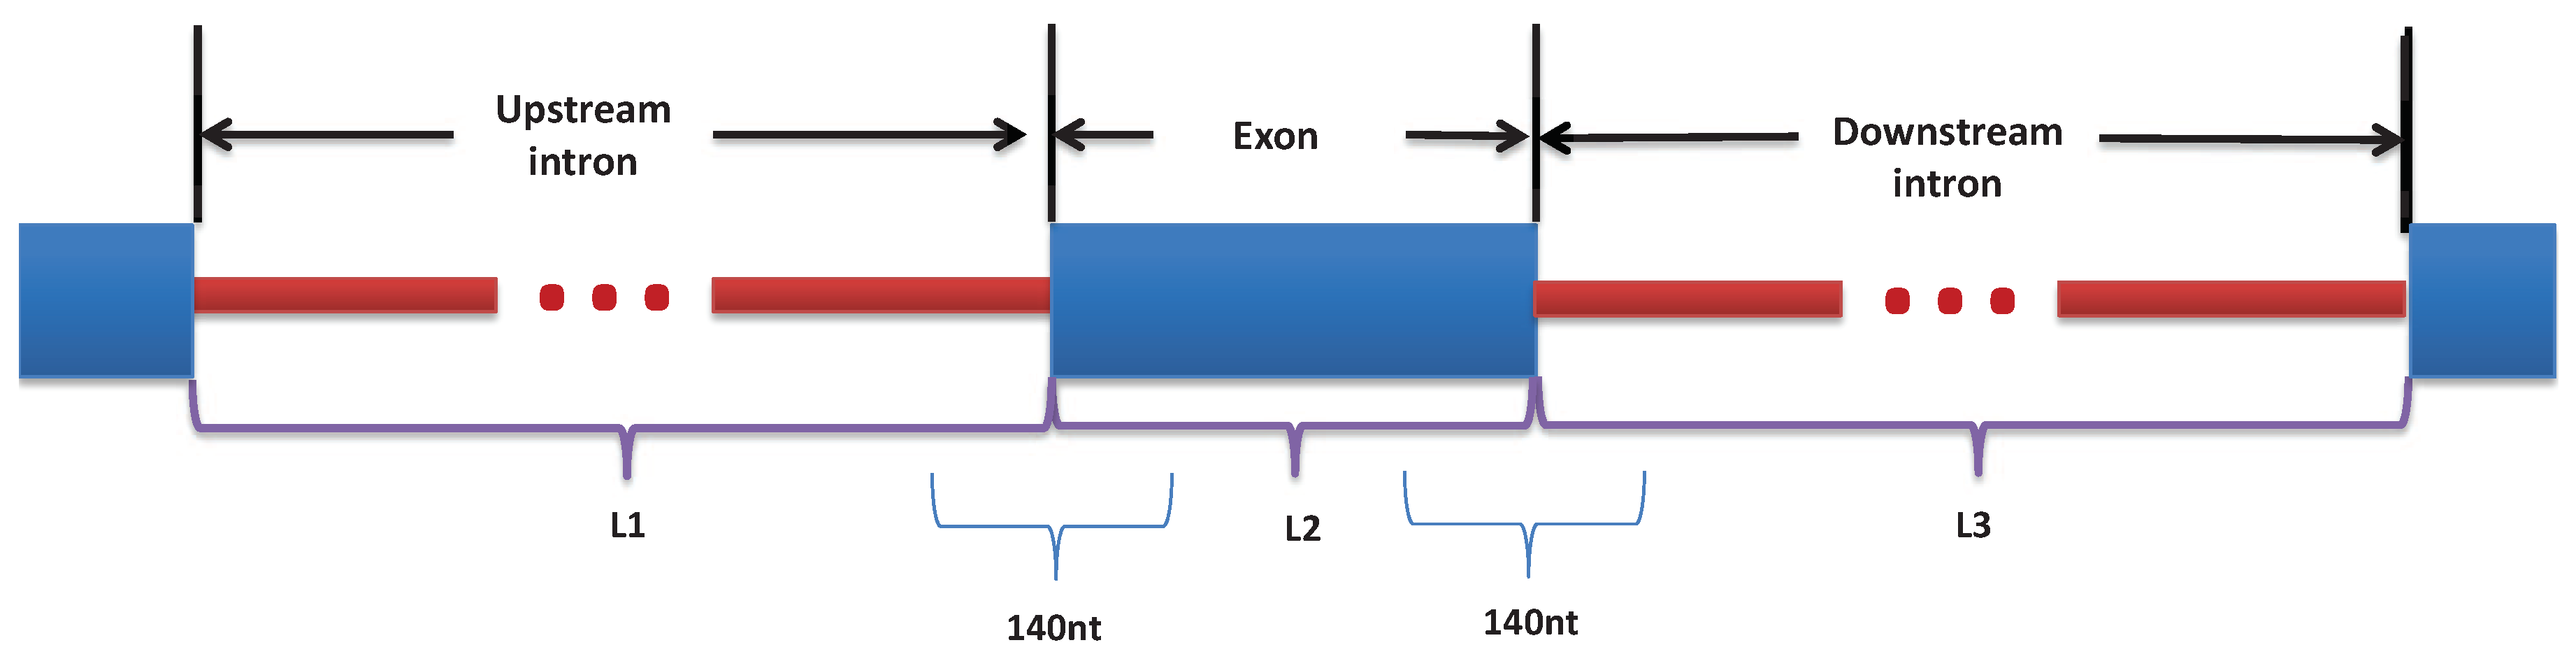
\includegraphics[width=0.9\textwidth]{../visualizations/ch4-methods/input_schematic.png} 
	\caption{Schematic of model input for an exon-centric training sample \cite{dsc}. The input are the 140 nucleotide region extracted around the exon start and exon end, as well as the normalized length of the exon and its flanking introns. The input for intron-centric training samples is analogue.}
	\label{fig:inputschematic}
\end{figure}

At this point, the datasets have been preprocessed such that we have the following information for each training sample that we want to create: 
\begin{itemize}
	\item chromosome and strand information of the to-be-used exon or junction,
	\item start and end coordinates of the exon or junction within a chromosome,
	\item the lengths of neighbouring introns or exons\footnote{Due to data limitations, we don't know the length of neighbouring exons when creating intron-centric training samples from GTEx data. In this case, the length of the neighbouring exons is set to 0. }.
\end{itemize}

Using this information, now either exon-centric or intron-centric training samples are created. Exon-centric training samples are created when the task of the network is to classify an exon or regress its PSI. Intron-centric training samples are created when the task of the network is to classify a junction or regress its PSI. 


Note that for intron-centric training samples we do not classify the intron or regress its PSI because the respective PSI is estimated with respect to the inclusion or exclusion of a particular junction. To estimate the PSI of an intron it would be necessary to also account for all other junctions which correspond to a particular intronic region being spliced in or not. 

%It wouldn't be accurate to say that 
%because a particular intronic sequence may be spliced out when 
%Note that it is not technically correct to say that we classify an intron or regress its PSI because the inclusion or exlusion of an intronic sequence may occur when 


Using the chromosome information, and the start and end coordinates, two 140 nucleotide window around the start and end coordinates were extracted from the human reference genome GRCh38 (see Figure \ref{fig:inputschematic}). The size of the nucleotide window was motivated by previous work \cite{dsc}. We refer to this input as the sequence input or sequence features. We abbreviate the sequence around the exon (or junction) start as start sequence. We define the end sequence analogue. 

Furthermore, if an exon or junction is taken from a negative strand, the extracted start and end windows are switched, the order of the nucleotides within the start and end windows are reversed and each extracted nucleotide is converted to its reverse complement. This mirrors biology, as the spliceosome also observes the exon start and end sites as switched and reverse complemented between the + and - strand.

%Presumably, this means the models don't have to learn different features for exons or junctions on the + and - strand. \\
Samples from the chromosomes X, Y and M were excluded due to the fundamental functional differences between them and the autosomes (e.g. there only exists one functional copy of the sex chromosomes).

The extracted nucleotides were one-hot encoded as four dimensional vectors. Specifically, adenine `A' is encoded as [1 0 0 0], cytosine `C' as [0 1 0 0], guanine `G' as [0 0 1 0] and thymine `T' as [0 0 0 1]. Thus, each 140 nucleotide long window was converted into an 140x4 matrix containing one-hot encoded nucleotides. 

It is commonplace that repetitive sequences are soft-masked as lower case letters in the reference genome. As this has no known bearing on alternative splicing, this information was ignored during one-hot encoding.

As in previous work \cite{dsc} \cite{flawed4}, we include the lengths of flanking exons or intron and the length of the exon or intron itself as additional input features. For brevity, we often refer to these exon and intron lengths as the length features. The inclusion of the length features is motivated by the observation that exon and intron lengths are correlated with splicing behaviour \cite{lengthsref1} \cite{lengthsref2}. In particular, alternatively spliced exons tend to be flanked by longer introns. This may be due to long intronic sequences making it more challenging for the spliceosome to locate the exon or it plainly being more likely that novel exons originate within long introns \cite{bestlengthsref}. 

%In addition to sequence information, the lengths of neighbouring introns or exons, as well as the length of the exon itself, are given as input to the models. Several studies have shown that exon and intron lengths can influence splice-site recognition. [15,34] In addition, previous studies have shown that including the length information dramatically model performance. [DSC] 

Introns are on average one to two orders of magnitudes larger than exons and their relative standard deviation is three times as large as that of exons. To avoid giving features to the network whose magnitude might differ by several orders of magnitude, the intron and exon lengths features were respectively normalized by the mean length and standard deviations of internal exons ($\mu=145, \sigma=198$) and introns ($\mu=5340, \sigma=17000$) in the human genome \cite{exonintronlens} \cite{bionumbers}. 

Some of the datasets contain significantly more constitutive, than non-constitutive training samples. For instance, the HexEvent dataset contains roughly three times as many constitutive as alternatively spliced samples. In these cases, we rebalanced the datasets by including each alternatively spliced sample multiple times until the class imbalance was less than two-to-one. 

%This leads to the issues with models getting stuck in local minima where they just predict the majority class. This was alleviated by including each alternatively spliced sample multiple times until the classes were balanced.

The end result is that a single training sample for the model contains two 140x4 one-hot encoded matrixes and three normalized length values. This is the model input.
The associated training label for the classification task is the scalar 1 if the respective exon or junction is constitutive, and 0 if not. The associated training label for the regression task is the PSI estimate. 
\subsection{Dataset statistics} \label{subsec:datasetstatistics}

%\begin{table}[h!]
%	\centering
%	\begin{tabular}{l | c c | c c c} 
%		%   \hline
%		\toprule
%		Name & Tissue & Type & Number of samples\\
%		%   \hline
%		\toprule
%		HEXEvent & mixed & exon & 50,918 \\
%		\hline
%		GTEx & brain cortex & exon & 30,466\\
%		GTEx & cerebellum & exon & 37,095\\
%		GTEx & heart & exon & 19,257\\
%		\hline
%		GTEx & brain cortex & intron & 127,908\\
%		GTEx & cerebellum & intron & 161,310\\
%		GTEx & heart & intron & 81,659\\
%		%   \hline
%		\hline
%		%   GTEx HEXEvent Reconstruction & brain & exon & 28,952\\
%		%   \hline
%		HipSci SUPPA & neuron & exon & 17,863 \\
%		HipSci MAJIQ & neuron & exon & 44,746 \\
%		HipSci MAJIQ & iPSC & exon & 48,652 \\
%		%   \hline
%		\hline
%		
%		%   GTEx HEXEvent Reconstruction & brain & junction & 57,201\\
%		%   HipSci MAJIQ & neuron & junction & 90,627 \\
%		%   \hline
%	\end{tabular}
%	\caption{Type, tissue and number of training samples per dataset. Type refers to whether the dataset is intron- or exon-centric.
%	}
%	\label{table:datasets}
%\end{table}

\begin{table}[h!]
	\centering
	\begin{tabular}{l | c c c | c c} 
		%   \hline
		\toprule
		Name & Tissue & Type & Misc & Number of samples\\
		%   \hline
		\toprule
		HEXEvent & mixed & exon & / & 50,918 \\
		\hline
		GTEx & brain cortex & exon & / & 30,466\\
		GTEx & cerebellum & exon & / & 37,095\\
		GTEx & heart & exon & / & 19,257\\
		\hline
		GTEx & brain cortex & intron & / & 127,908\\
		GTEx & cerebellum & intron & / & 161,310\\
		GTEx & heart & intron & / & 81,659\\
		%   \hline
		\hline
		%   GTEx HEXEvent Reconstruction & brain & exon & 28,952\\
		%   \hline
		HipSci SUPPA & neuron & exon & / & 17,863 \\
		\hline
		HipSci MAJIQ & neuron & exon & / & 44,746 \\
		HipSci MAJIQ & iPSC & exon & / & 48,652 \\
		HipSci MAJIQ & iPSC & exon & diff lib & 49,275 \\
		HipSci MAJIQ & iPSC & exon & diff indv & 48,489 \\
		
		%   \hline
		\hline
		
		%   GTEx HEXEvent Reconstruction & brain & junction & 57,201\\
		%   HipSci MAJIQ & neuron & junction & 90,627 \\
		%   \hline
	\end{tabular}
	\caption{Type, tissue and number of training samples per dataset. Type refers to whether the dataset is intron- or exon-centric. `diff lib' abbreviates that the dataset was taken from the same individual, but a different library and `diff indv' abbreviates that the dataset was taken from a different individual than the first shown HipSci MAJIQ iPSC cell-based dataset. 
	}
	\label{table:datasets}
\end{table}
% add more statistics now; decision to show the junction results (as majiq also does modelling predominantly on junctions), as i can say that my gtex dataset will have constitutive junctions and no issue with misattributed reads; number of reads

Table \ref{table:datasets} shows the number of training samples in each dataset.%\footnote{We omit the HipSci MAJIQ iPSC cell-based datasets from a different library, but the same individual and from a different individual. We give the complete table in the appendix \ref{app:datasets} } 
%Among the exon-centric datasets, the HEXEvent dataset contains the most samples, followed by the HipSci MAJIQ, GTEx and HIPSCI MAJIQ datasets. 
Among the exon-centric datasets, the HEXEvent and HipSci MAJIQ datasets contain comparatively more training samples because they also contain constitutive non-cassette exons, whereas the other datasets don't. In contrast to the sensory neuron and iPSC cell-based HipSci datasets, the magnitudes of the GTEx-based datasets vary a lot between tissues: the cerebellum tissue dataset contains roughly twice as many training samples as the heart tissue dataset. 
On closer investigation, this is because the cerebellum tissue contains 10,000 genes whereas the heart sample only contains 5,000. Surprisingly, the heart tissue is based on 17 million exon-exon junction reads compared to 8 million exon-exon junction reads from the cerebellum tissue sample. The additional reads from the heart sample are concentrated in a few extremely highly expressed genes (e.g. gene ENSG00000198886 is expressed 1000-times as often as the median highly expressed gene) and while this concentration of reads also appear in the cerebellum tissue, it is less extreme.

The same cross-tissue observations also hold for the intron-centric GTEx-based datasets. In general, the intron-centric datasets contain roughly four times more training samples than the exon-centric datasets. This is because they do not only contain junctions of cassette exons (in which case they would contain roughly twice as many training samples as the exon-centric datasets) but contain all non-filtered junctions. 
% ENSG00000198886 - MT-ND4 - https://www.proteinatlas.org/ENSG00000198886-MT-ND4
%
%ENSG00000198899 - MT-ATP6 - https://www.proteinatlas.org/ENSG00000198899-MT-ATP6/tissue - very highly expressed in blood
%ENSG00000198712 - MT-CO2 - https://www.proteinatlas.org/ENSG00000198712-MT-CO2/tissue - very highly expressed in blood / muscle tissues
%ENSG00000198804 - MT-CO1 - https://www.proteinatlas.org/ENSG00000198804-MT-CO1/tissue - very high muscle yep



%gtex number of reads:
%The initial dataset contained roughly 10 million total exon-exon junction read count for each tissue distributed over roughly 330,000 unique junctions.

\begin{figure}
	\centering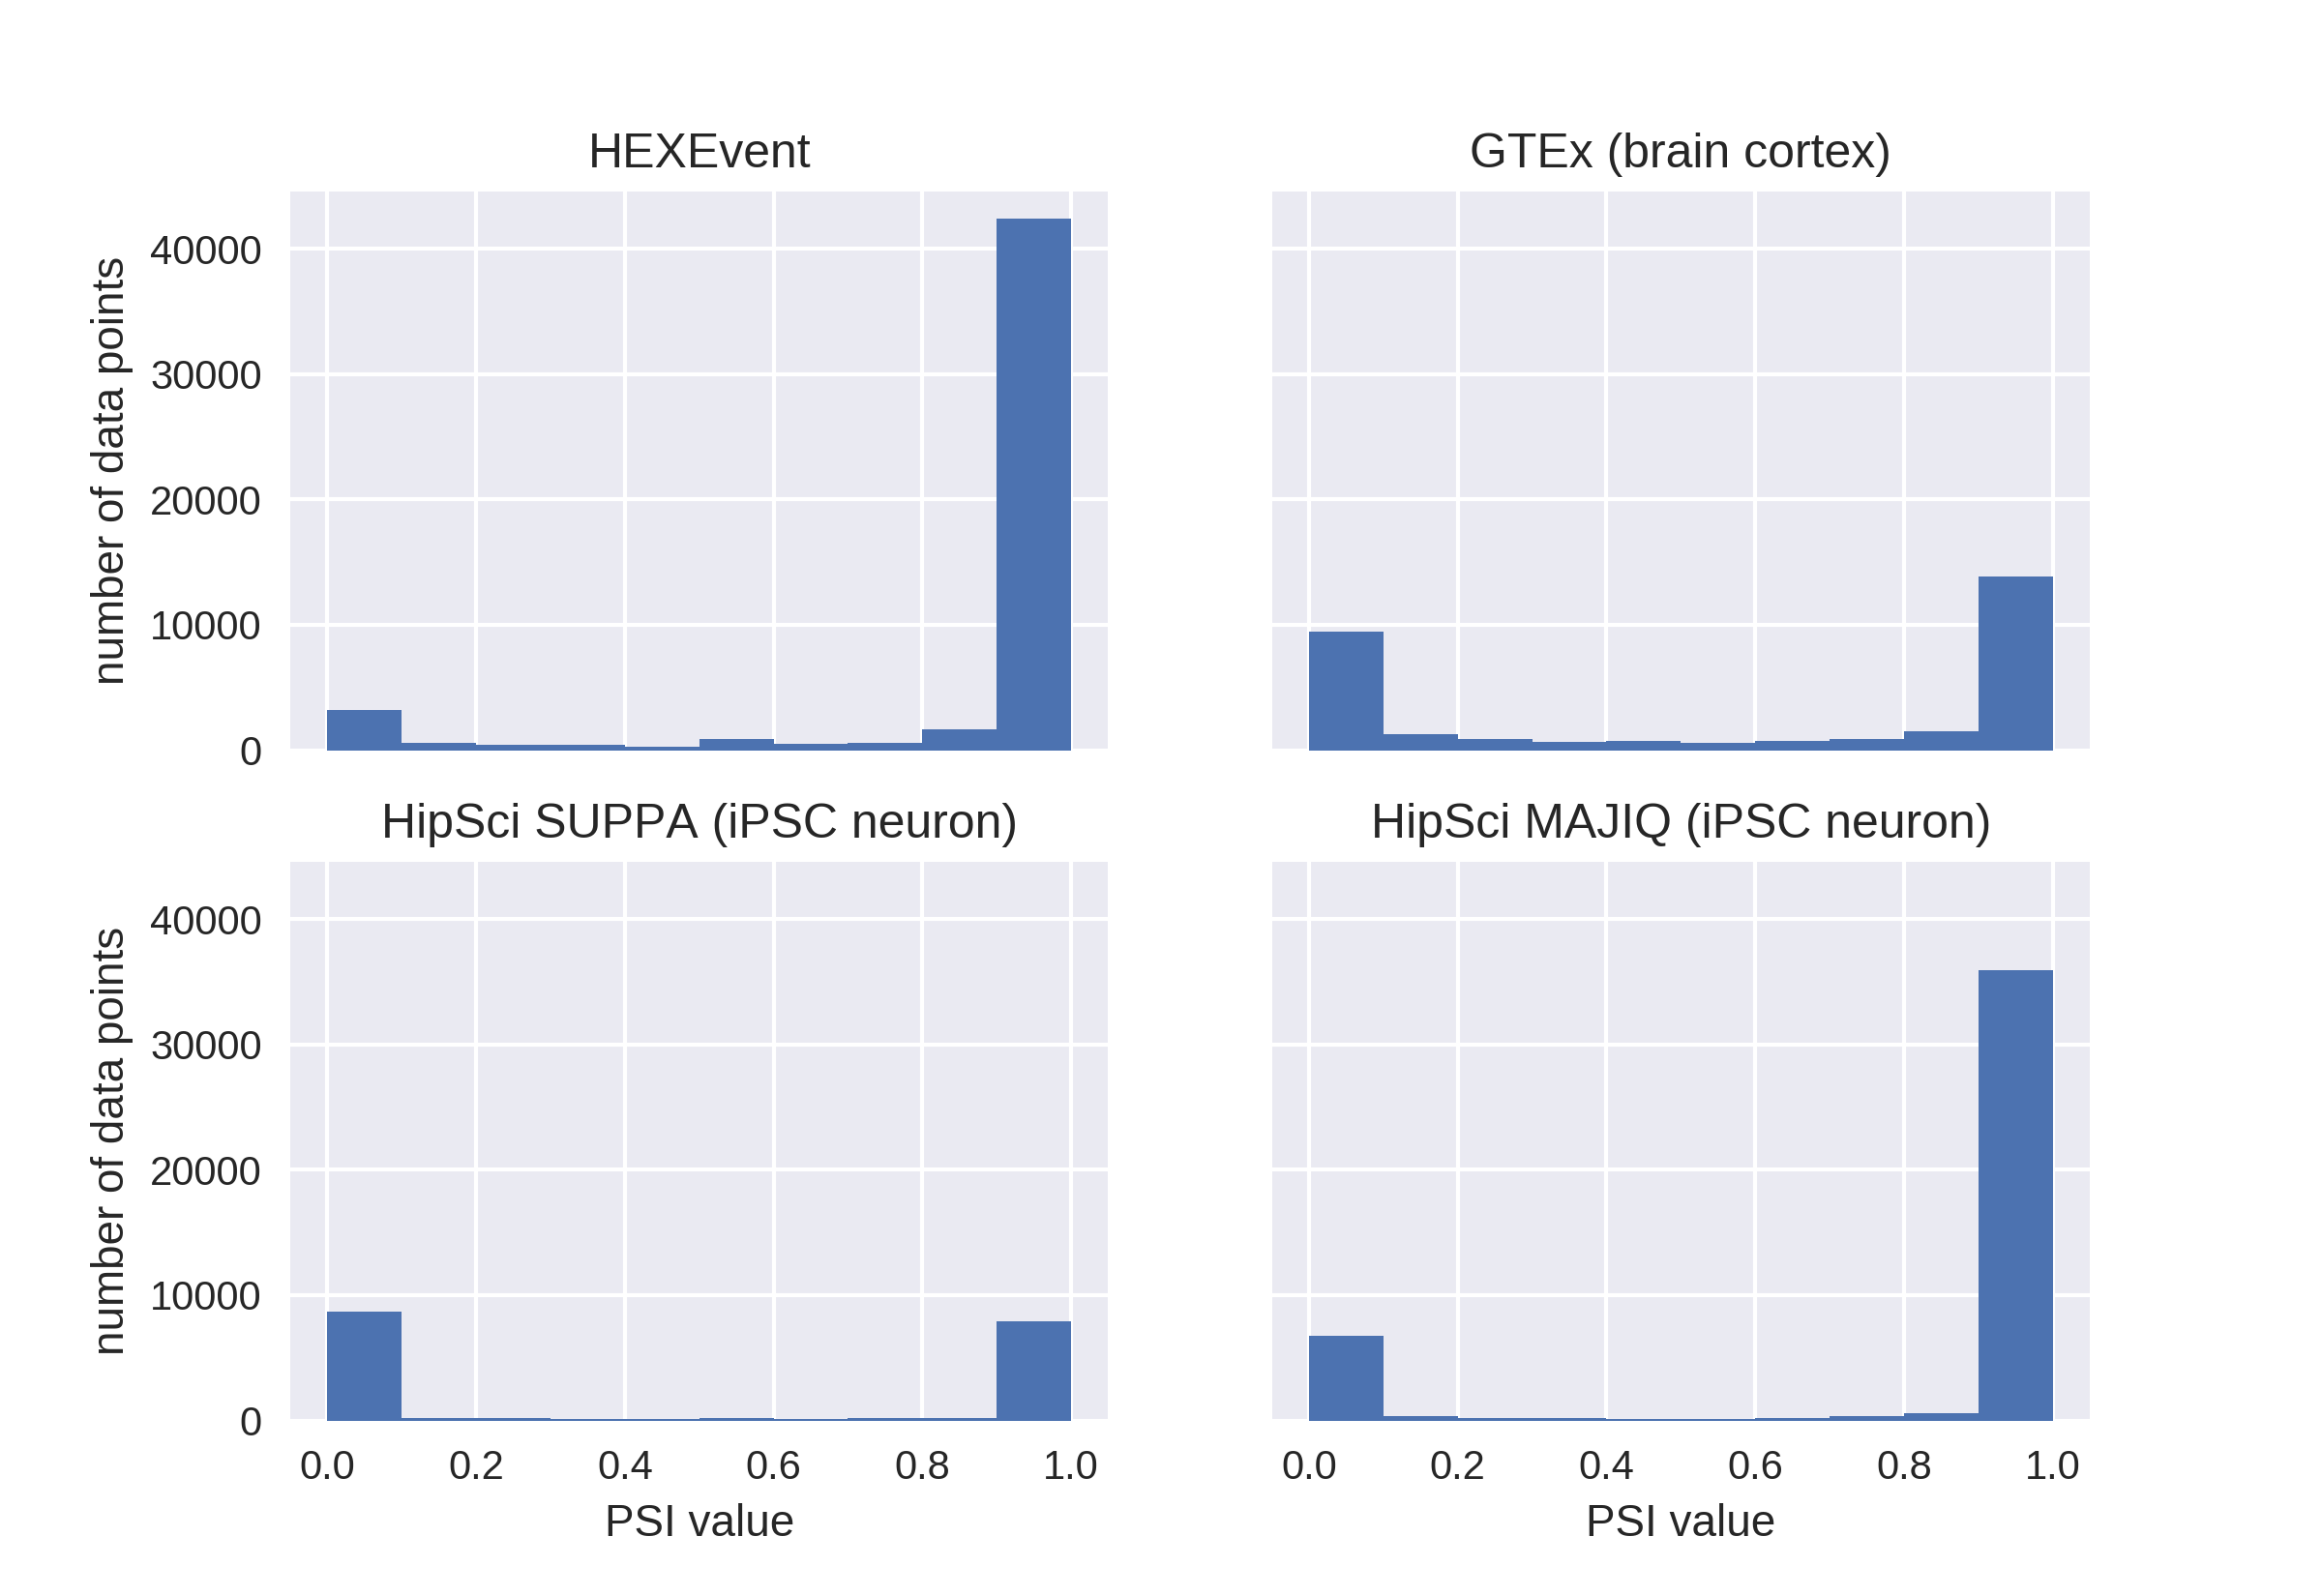
\includegraphics[width=1\textwidth]{../visualizations/ch4-methods/dataset_histograms_seaborn.png} 
	\caption[test.]{
		Histograms comparing the exon-centric versions of the four fundamentally different training datasets used. The shown GTEx dataset is based on samples from brain cortex tissue and the shown HipSci datasets are based on samples from iPSC cells differentiated to neurons. 
	}
	\label{fig:datahistograms}
\end{figure}

Figure \ref{fig:datahistograms} shows histograms for the exon-centric version of the four primary datasets versions. The histograms show that in each dataset the distribution of PSI values is bi-modal with modes around very rarely included (< 5\%) and very frequently included exons (>95\%). This aligns well with previous observations that alternatively spliced junctions and exons tend to be very frequently or very rarely included \cite{buschhertel} \cite{bimodalpsivalues1} \cite{bimodalpsivalues2}.\\
The lack of non-cassette constitutive exons is visible in the GTEx and HipSci SUPPA datasets containing significantly fewer constitutive samples; the other two primary datasets contain roughly three times as many constitutive as non-constitutive samples. \\
% However, there are also some dissimilarities between the datasets: the GTEx and HipSci SUPPA dataset contain the fewest samples and, in particular, they contain significantly fewer constitutive samples.\\
%Due to their respective processing methods the GTEx and HipSci SUPPA datasets only contain known cassette exons as constitutive exons, but not non-cassette constitutive exons. 
% liekly false for suppa Another factor is that they only estimate PSI based on one biological sample in contrast to the other datasets. 
In particular, the HipSci SUPPA dataset contains an extremely low number of non-rarely or frequently included exons (only $\sim$1\%) which is likely an artefact of its coarse, transcription-level estimation method.
%The relatively low number of non-constitutive exon samples in the HEXEvent dataset is likely influenced by the ESTs coming from a mix of biological samples from different tissues. Among many tissues, there are likely few tissues that contain some exons
%should also hold for constitutive exons; so rarely exons constitutive, so more with middle psi values
%SCEPTICAL -- unlikely to include

\section{Models} \label{sec:models}
All three models are fundamentally split into two components: 
\begin{enumerate}
	\item The first component extracts the most relevant features of the two input sequences of nucleotides.  Depending on the exact model, the feature extraction is based either on Convolutional Neural Networks (CNNs), word embeddings or Bidirectional Long-Short Term Memory Units (BiLSTMs) and an attention layer. The extracted features are concatenated along with the length features and fed as input to the second component. 
	
	\item The second component uses the extracted features and length features to perform binary classification or regression. This component is implemented as a shallow multilayer perceptron (MLP) for all models. It consists of one or two fully connected layers followed by dropout and activation layers. A sigmoid activation function is used after the last layer to obtain an output between 0 and 1.
\end{enumerate}

\subsection{DSC: CNN-based} \label{subsec:dsc}
This model is a reimplementation of the Deep Splicing Code (DSC) from \cite{dsc} and the current state-of-the-art model for the classification of alternative splicing events. 

\begin{figure}
	\centering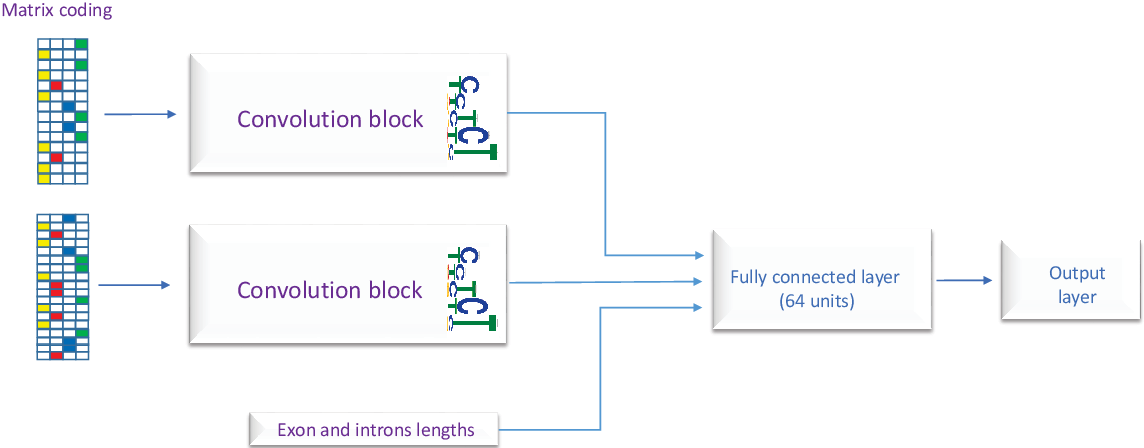
\includegraphics[width=1\textwidth]{../visualizations/ch4-methods/dsc_architecture.png} 
	\caption{
		Architecture of DSC \cite{dsc}. 
		%		The one-hot encoded sequences are fed into two convolutional blocks which generate features that are concatenated with the exon and intron lengths. The sequence and length features are then used by a fully-connected layer to obtain the classification output.
	}
	\label{fig:dsc_architecture}
\end{figure}

\subsubsection{The motivation behind using CNNs}
DSC uses CNNs for feature extraction. 
CNNs are useful when the input data contains spatially invariant patterns.  Since images are fundamentally made up of small, spatially invariant patterns which can be combined into more complex patterns, CNNs have been extremely successful in Computer Vision.
CNNs are also promising for the application to genomic data: 
\begin{itemize}
	\item Nucleotide sequences contain motifs (nucleotide sequence patterns conjectured to be biologically significant). Motifs are frequently represented as position weight matrixes (PWMs) which encode information about the significance of the occurrence of a particular nucleotide at a particular position. The kernels used in CNNs can be interpreted as PWMs with learnable weights. Thus, the inductive bias of CNNs, that the learning task can be solved via optimizing matrix weights, aligns well with our initial knowledge about the task. %  are promising because they can automatically optimize these weights and learn to recognize important motifs.
	\item Motifs are found at different positions in the input sequence. This isn't a natural problem setting for some Machine Learning algorithms since they would need to learn to recognize the same motif in different positions. However, CNNs are inherently spatially invariant and thus are again well-suited to detecting motifs within a sequence.
\end{itemize}


\subsubsection{Model architecture}
Keeping this motivation in mind, DSC extracts features from the two input sequences using CNN-based blocks. A CNN feature extraction block with the same architecture but independently learned weights are used for each input sequence. This is to accommodate the model learning to extract different features from the exon start and exon end sequence. The extracted features are concatenated with the lengths and used by a shallow MLP for predicting the output. The architecture of DSC is visualized in \ref{fig:dsc_architecture}.

Concretely, each CNN block consists of three convolutional layers. The first convolutional layer has a window size of 7 units and 32 filters, the second has a window size of 4 units and 8 filters and the third has a window size of 3 units and 8 filters. Each convolutional layer is followed by a dropout layer with dropout probability 0.2 to reduce overfitting \cite{dropout}, a ReLU activation layer \cite{relu} and a max-pooling layer with stride and window size 2 to extract the most salient features. The hyperparameters for this model were chosen with grid search by \cite{dsc}. 1D convolution layers are used. 
%In contrast to images from Computer Vision, sequences from genomics are 1-dimensional, and  
%As we are dealing with 1-dimensional textual data instead of inherently 2-dimensional image data, 1D convolution layers are used.



%https://stats.stackexchange.com/questions/288261/why-is-max-pooling-necessary-in-convolutional-neural-networks
%no one knows why max-pooling works

%The extracted features for both genomic sequences are concatenated along with the normalized exon and flanking introns and input to a fully connected layer with 64 neurons. A ReLU activation function, as well as a dropout layer with probability 0.5, is applied to the output of this layer. The final layer takes in the 64 outputs from the previous layer, predicts a single value and is followed by a sigmoid activation layer.

\subsubsection{Applying NLP techniques to genomic data}
Like text, genomic data is fundamentally a sequence of characters.
This makes it possible to apply techniques known from NLP to genomic data. This is an especially promising area of cross-pollination because of the large strides NLP has been able to make in recent years using Deep Learning.
Some of the most important milestones in NLP have been efficient embeddings via Word2Vec \cite{w2v1} \cite{w2v2}, applying Recurrent Neural Networkss (RNNs) to text as in Sequence-to-Sequence (seq2seq) learning \cite{seq2seq} and leveraging attention as in the extremely powerful and deep Transformer models \cite{allyouneed} \cite{bert}.\\
In this work, we evaluate the application of Doc2Vec (a derivative of Word2Vec), Seq2Seq models and the attention mechanism for the classification of alternative splicing events and the regressing of their frequency. We don't evaluate the current state-of-the-art Transformer models. Albeit very potent, they usually require huge datasets in the order of millions of samples which aren't available for this task (this decision is discussed in more detail in Section \ref{lstmvstransformer}). Nonetheless, we do adapt the attention mechanism as known from Transformers for our task. In this way, we feel the evaluated models make use of the most important Deep Learning innovations originating from NLP.

%While scaling down Transformers and then applying is an interesting avenue of research, even heavily scaled-down models might still be over parametrized for the task as it has frequently been shown that very shallow networks (with less than 5 layers) perform best on genomic data \cite{}. Additionally, our input sequences are very long; generally 140 tokens or more. Initial tests showed that this also leads to memory problems when training on only one GPU, as the memory requirements of Transformers grows quadratically with respect to the length of the input sequence, further complicating their application. Due to these considerations, we chose to forego the evaluation of Transformer-based models in this study.
\subsection{D2V: MLP-based} \label{subsec:d2v}
This model is a reimplementation of the model used for PSI regression on the mouse genome in \cite{d2vsplicing}. The only architectural difference is that we possibly use a differently-sized MLP in the second part of the network, as architectural details on the MLP aren't given and no public implementation is available. 
%If I want to expand this section:
%Asgari, E., & Mofrad, M. R. (2015). Continuous distributed representation of biological sequences for deep proteomics and genomics. PloS one, 10(11), e0141287.
%Contains very good explanations / phrasings
\subsubsection{Introduction to word embeddings}
Word2Vec is a neural network-based model which provides a continuously distributed (vector) representation for each word within a sentence \cite{w2v1}\cite{w2v2}. The representation is chosen so that semantically and syntactically similar words have similar representations. The key idea through which Word2Vec achieves this is by representing words based on the context they appear in. To obtain the word representations, a shallow neural network is trained on a large corpus of unlabelled text with a loss which incentivizes the model to learn such a representation.

Trained Word2Vec models have been shown to recover semantic and syntactic relationships. Keeping in mind that each word is represented as a numerical vector, the following equation usually holds on trained Word2Vec models: 
$\vec{King} - \vec{Man} + \vec{Woman} \sim = \vec{Queen}$ 
where $\vec{x}$ represents the vector representation or embedding of word $x$.
% Since each word is represented as a numerical vector, mathematical operations can be applied to these vectors. In practice, Word2Vec recovers semantic relationships such as: 
%This works extremely well in practice and the representation of semantically related words is often similar. If Word2Vec is trained on a large corpus of text, then often one obtains equations such as 

%Distributed representation has proved one of the most successful approaches in machine learning [6–10]. The main idea in this approach is encoding and storing information about an item within a system through establishing its interactions with other members. [biobvec]



Doc2Vec is an extension of Word2Vec which uses the same principles, but can also handle variable-length texts (such as paragraphs and complete documents) \cite{d2v1} \cite{d2v2}. It returns a fixed-length representation independent of input size.

\subsubsection{Training}
To train Word2Vec or Doc2Vec, a large corpus of unlabelled data is needed. As we are training on genomic data, the largest corpus is the complete genome itself. To this end, we obtained the complete human reference genome GRCh38 from UCSC \cite{ucsc}.\\ %http://hgdownload.soe.ucsc.edu/goldenPath/hg38/chromosomes/
During training on text data, the corpus is split into documents which are ideally semantically meaningful (like paragraphs). Due to memory limitations and due to corresponding to the average gene size \cite{bionumbers}, we split the genome into sequences of 28,000 nucleotide sequences. Tests with splitting the genome into sequences of length 10,000 showed that the effect of this choice on model performance is imperceptible. 
%showed that the effect of this document length parameter on performance is negligible. 
%does not seem to affect model performance in a meaningful way.
\subsubsection{Using k-mers}\label{subsubsec:kmers}
Naively applying Word2Vec or Doc2Vec to genomic data would mean treating each nucleotide as a word. Drawing the parallel to natural language, this would mean wanting to embed each character in a word. However, a single character or nucleotide (which comes from an alphabet of only four characters) is not unique enough and occurs in too many contexts to obtain meaningful representations. Therefore, it is desirable to embed multiple characters or multiple sequences, that is a word or a k-mer. While a sentence can easily be split into words, the split of a nucleotide sequence into k-mers is not as clear-cut: we don't know the functionality of most nucleotides and therefore can't split a sequence into semantically meaningful units.

Previous studies have explored this issue \cite{kmerlength1} \cite{kmerlength2}, and found that the compromise of splitting each nucleotide sequence into overlapping 3-mers is a performant choice. Overlapping means that in the case of the sequence `AACGAT' the resulting overlapping 3-mer sequence is `AAC', `ACG', `CGA' and `GAT'. Based on these findings, we split each sequence of nucleotides into overlapping 3-mers and obtain 27,998 overlapping 3-mers from the 28,000 nucleotides long pre-training sequences. 

% Following this recommendation, we split the 28,000 nucleotides long pre-training sequences into 27,998 overlapping 3-mers.
\subsubsection{Pre-training of word embeddings}
The pre-training for Word2Vec and Doc2Vec uses a shallow neural network with one hidden layer. %During a pre-training epoch, each word is once in the centre of a sliding window or context window. 
One of two techniques is typically used for pre-training: either continuous bag-of-words (CBOW) or skip-gram. If CBOW is used, all words in a context window except the current word are given as input and the target output is the current word.  % [WHAT DOES THE HIDDEN LAYER LOOK LIKE? -- could honestly skip this]
If the skip-gram technique is used, only the current word is given as input and the task is to predict the surrounding words in the window. The context or sliding window around a word contains the words immediately adjacent to it. A typical window size is 5 words, meaning 5 words behind and after the current word will be used. 

Doc2Vec works similarly. In the CBOW equivalent called distributed memory (DM), a document identifier (commonly simply an integer enumerating all documents) is given as additional input. In the skip-gram equivalent distributed bag of words (DBOW), the current word is replaced by the document identifier and the task is to predict all words in the window. All four different training methods are visualized in Figure \ref{fig:w2vd2vtrainingvariants}.

There is no clear guideline for when which training method should be used for Word2Vec or Doc2Vec as they tend to perform similarly. However, DM (and also CBOW) preserve the order of words and as the order of words (3-mers) is likely significant, we chose DM as pre-training method.\\
Pre-processing the human genome like described above and using the DM training method, we trained a Doc2Vec model to output a 100-dimensional embedding for each document.
%\begin{figure}
%	\centering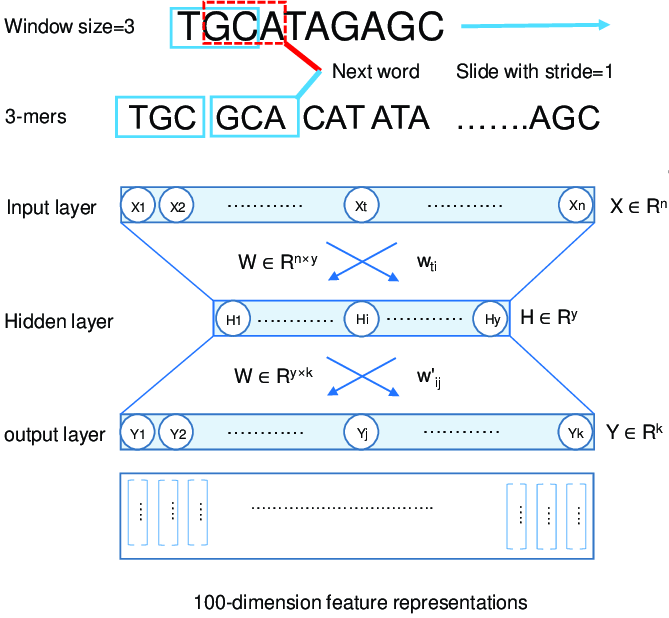
\includegraphics[width=1\textwidth]{../visualizations/ch4-methods/d2v_training_cropped.png} 
%	\caption{
%		Process by which the 100-dimensional embeddings are obtained \cite{d2vsplicing}: the input sequence is split into overlapping 3-mers which are then fed as input into the pre-trained d2v model. 
%		% add sentence how 100-dimensional embedding is actually obtained
%	}
%	\label{fig:d2vtraining}
%\end{figure}

\begin{figure}
	\centering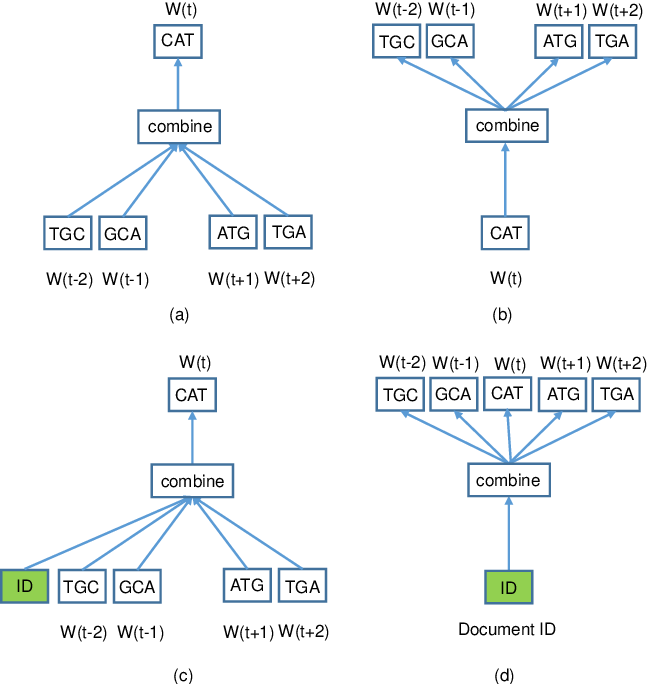
\includegraphics[width=0.7\textwidth]{../visualizations/ch4-methods/w2v_d2v_training_variants.png} 
	\caption{
		The four possible training algorithms for w2v and d2v models \cite{d2vsplicing}: (a) CBOW, and (b) skip-gram for w2v, and (c) DM and (d) DBOW for d2v. 
	}
	\label{fig:w2vd2vtrainingvariants}
\end{figure}

\subsubsection{Obtaing the embeddings}
After pre-training, the embedding for a given word or document is then the value of the hidden cells of the shallow pre-training MLP\footnote{In practice, the words in a corpus are one-hot encoded and the value of the hidden layers doesn't need to be computed. Recalling that the weights of the hidden layer of an MLP are represented as a $N\times d$ matrix, only the d-dimensional column which belongs to the respective one-hot encoded word needs to be retrieved. All other columns will be multiplied by 0. $N$ represents the size of the vocabulary (64 for us) and $d$ the number of embedding dimensions (100 for us).}. In the case of 100-dimensional embeddings, this means that the hidden layer contains 100 neurons. The intuition behind this is that the models learned a representation which is helpful for the prediction task the model was trained on. Since the prediction task was either to reconstruct a word or document given its context or vice-versa, the representation for a given word or document should encode its context. Thus, the main idea behind Word2Vec and Doc2Vec, that a word or document is defined by the context in which it occurs (and its representation should encode this context), is achieved.



\subsubsection{Analyzing the obtained embeddings}

%\begin{figure}
%	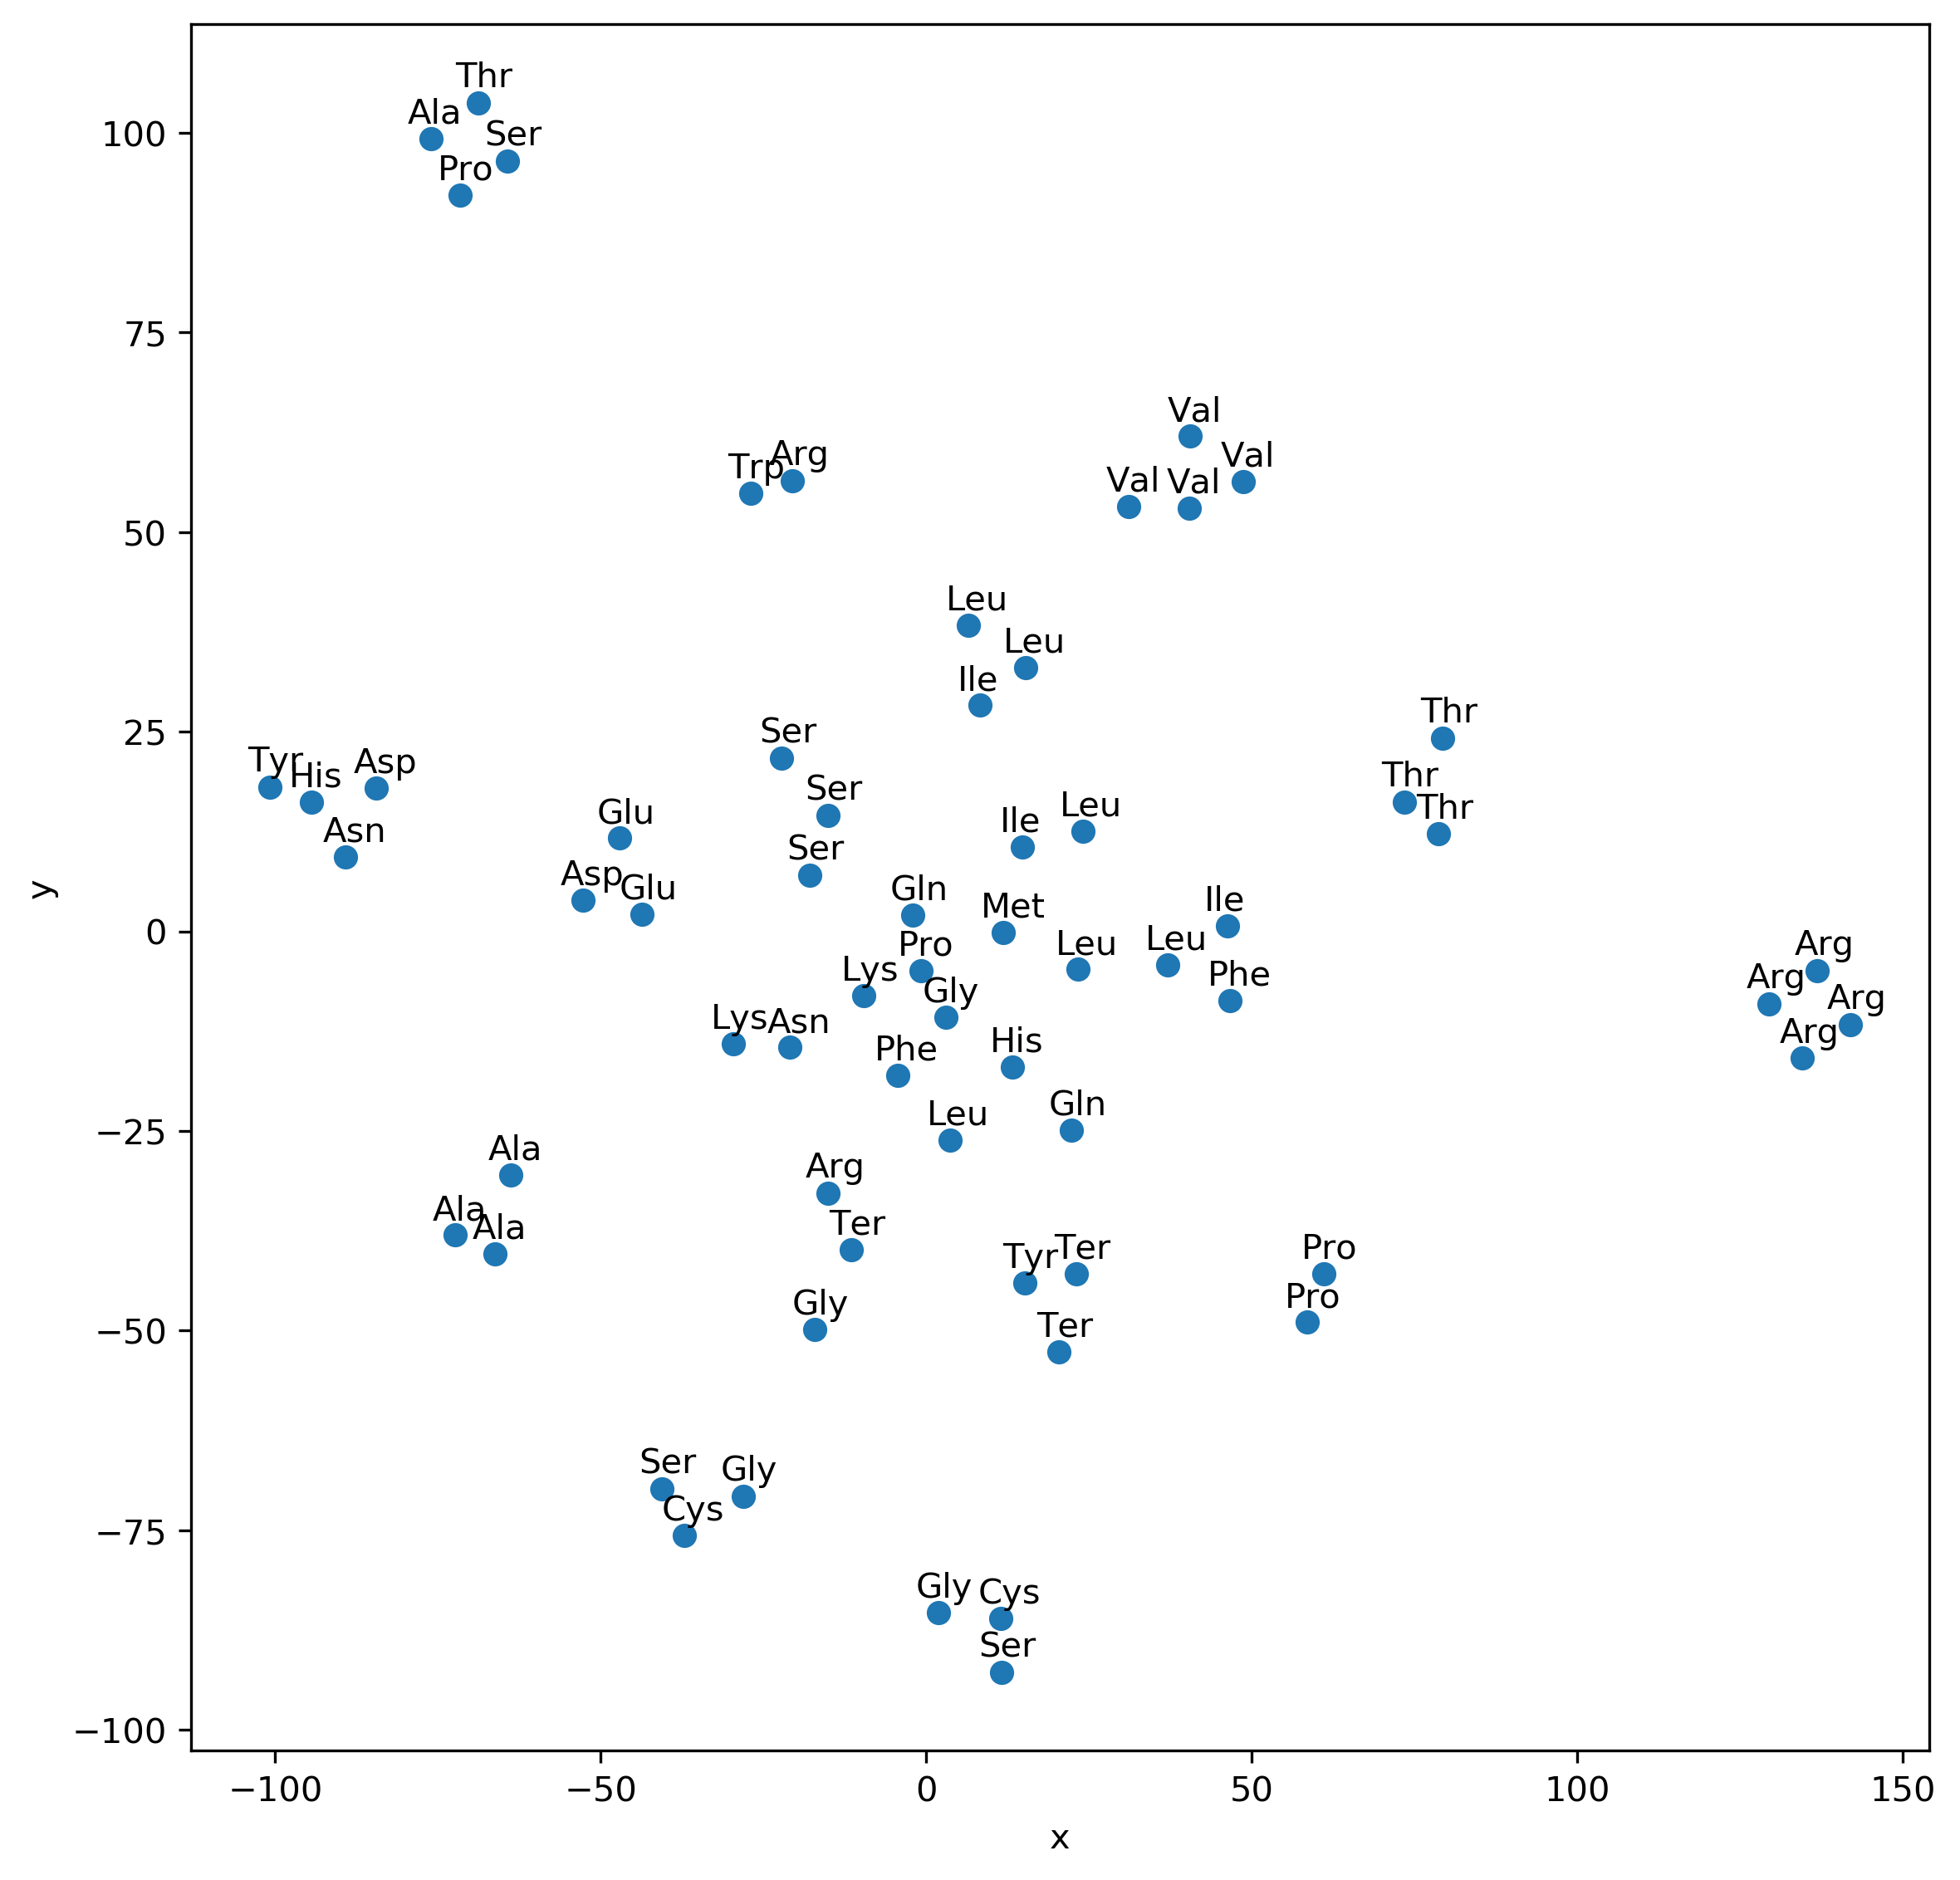
\includegraphics[width=0.5\textwidth]{../visualizations/ch4-methods/tSNE-d2v.png} 	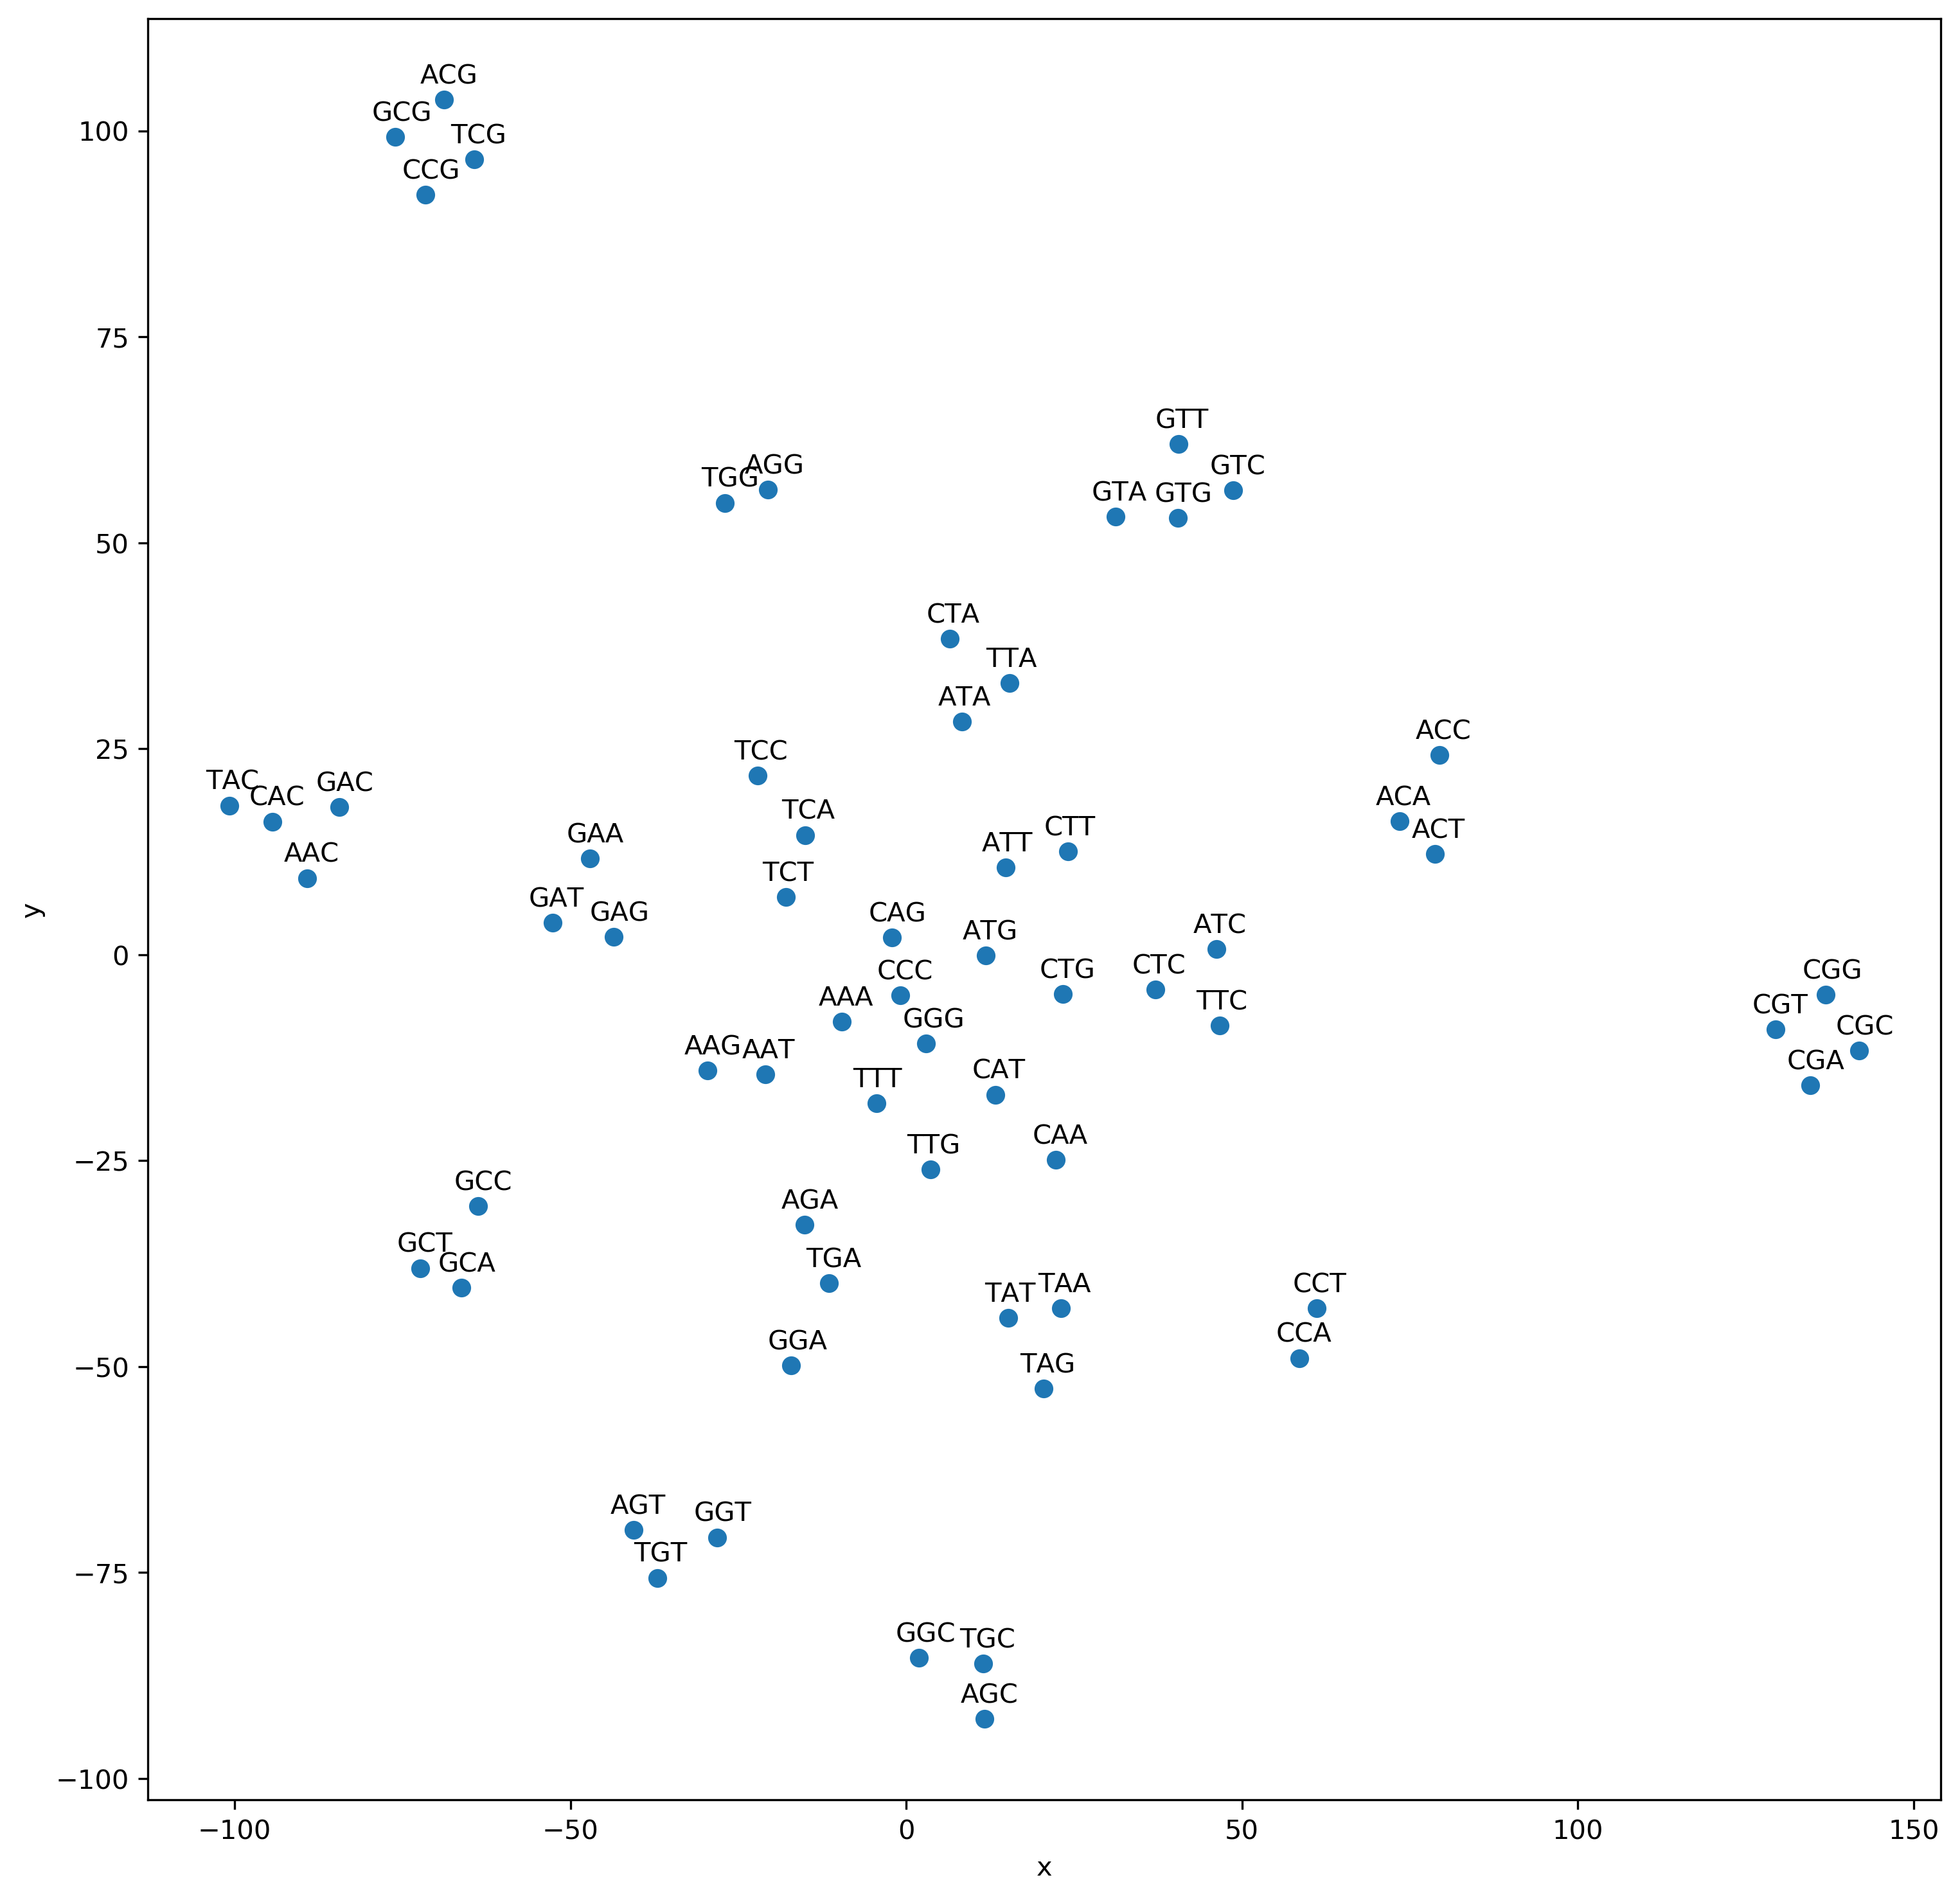
\includegraphics[width=0.5\textwidth]{../visualizations/ch4-methods/tSNE-d2v_bases.png} 
%	\caption{
%		The 2-dimensional embeddings obtained by applying t-SNE to the 100-dimensional learned representations of all 64 possible 3-mers. Left shows the codons encoded by the 3-mers, right shows the actual 3-mers.
%		 }
%%	 TODO: make this one picture where codons are color-coded but still labelledw ith 3-mers
%	\label{fig:tsne}
%\end{figure}

\begin{figure}
	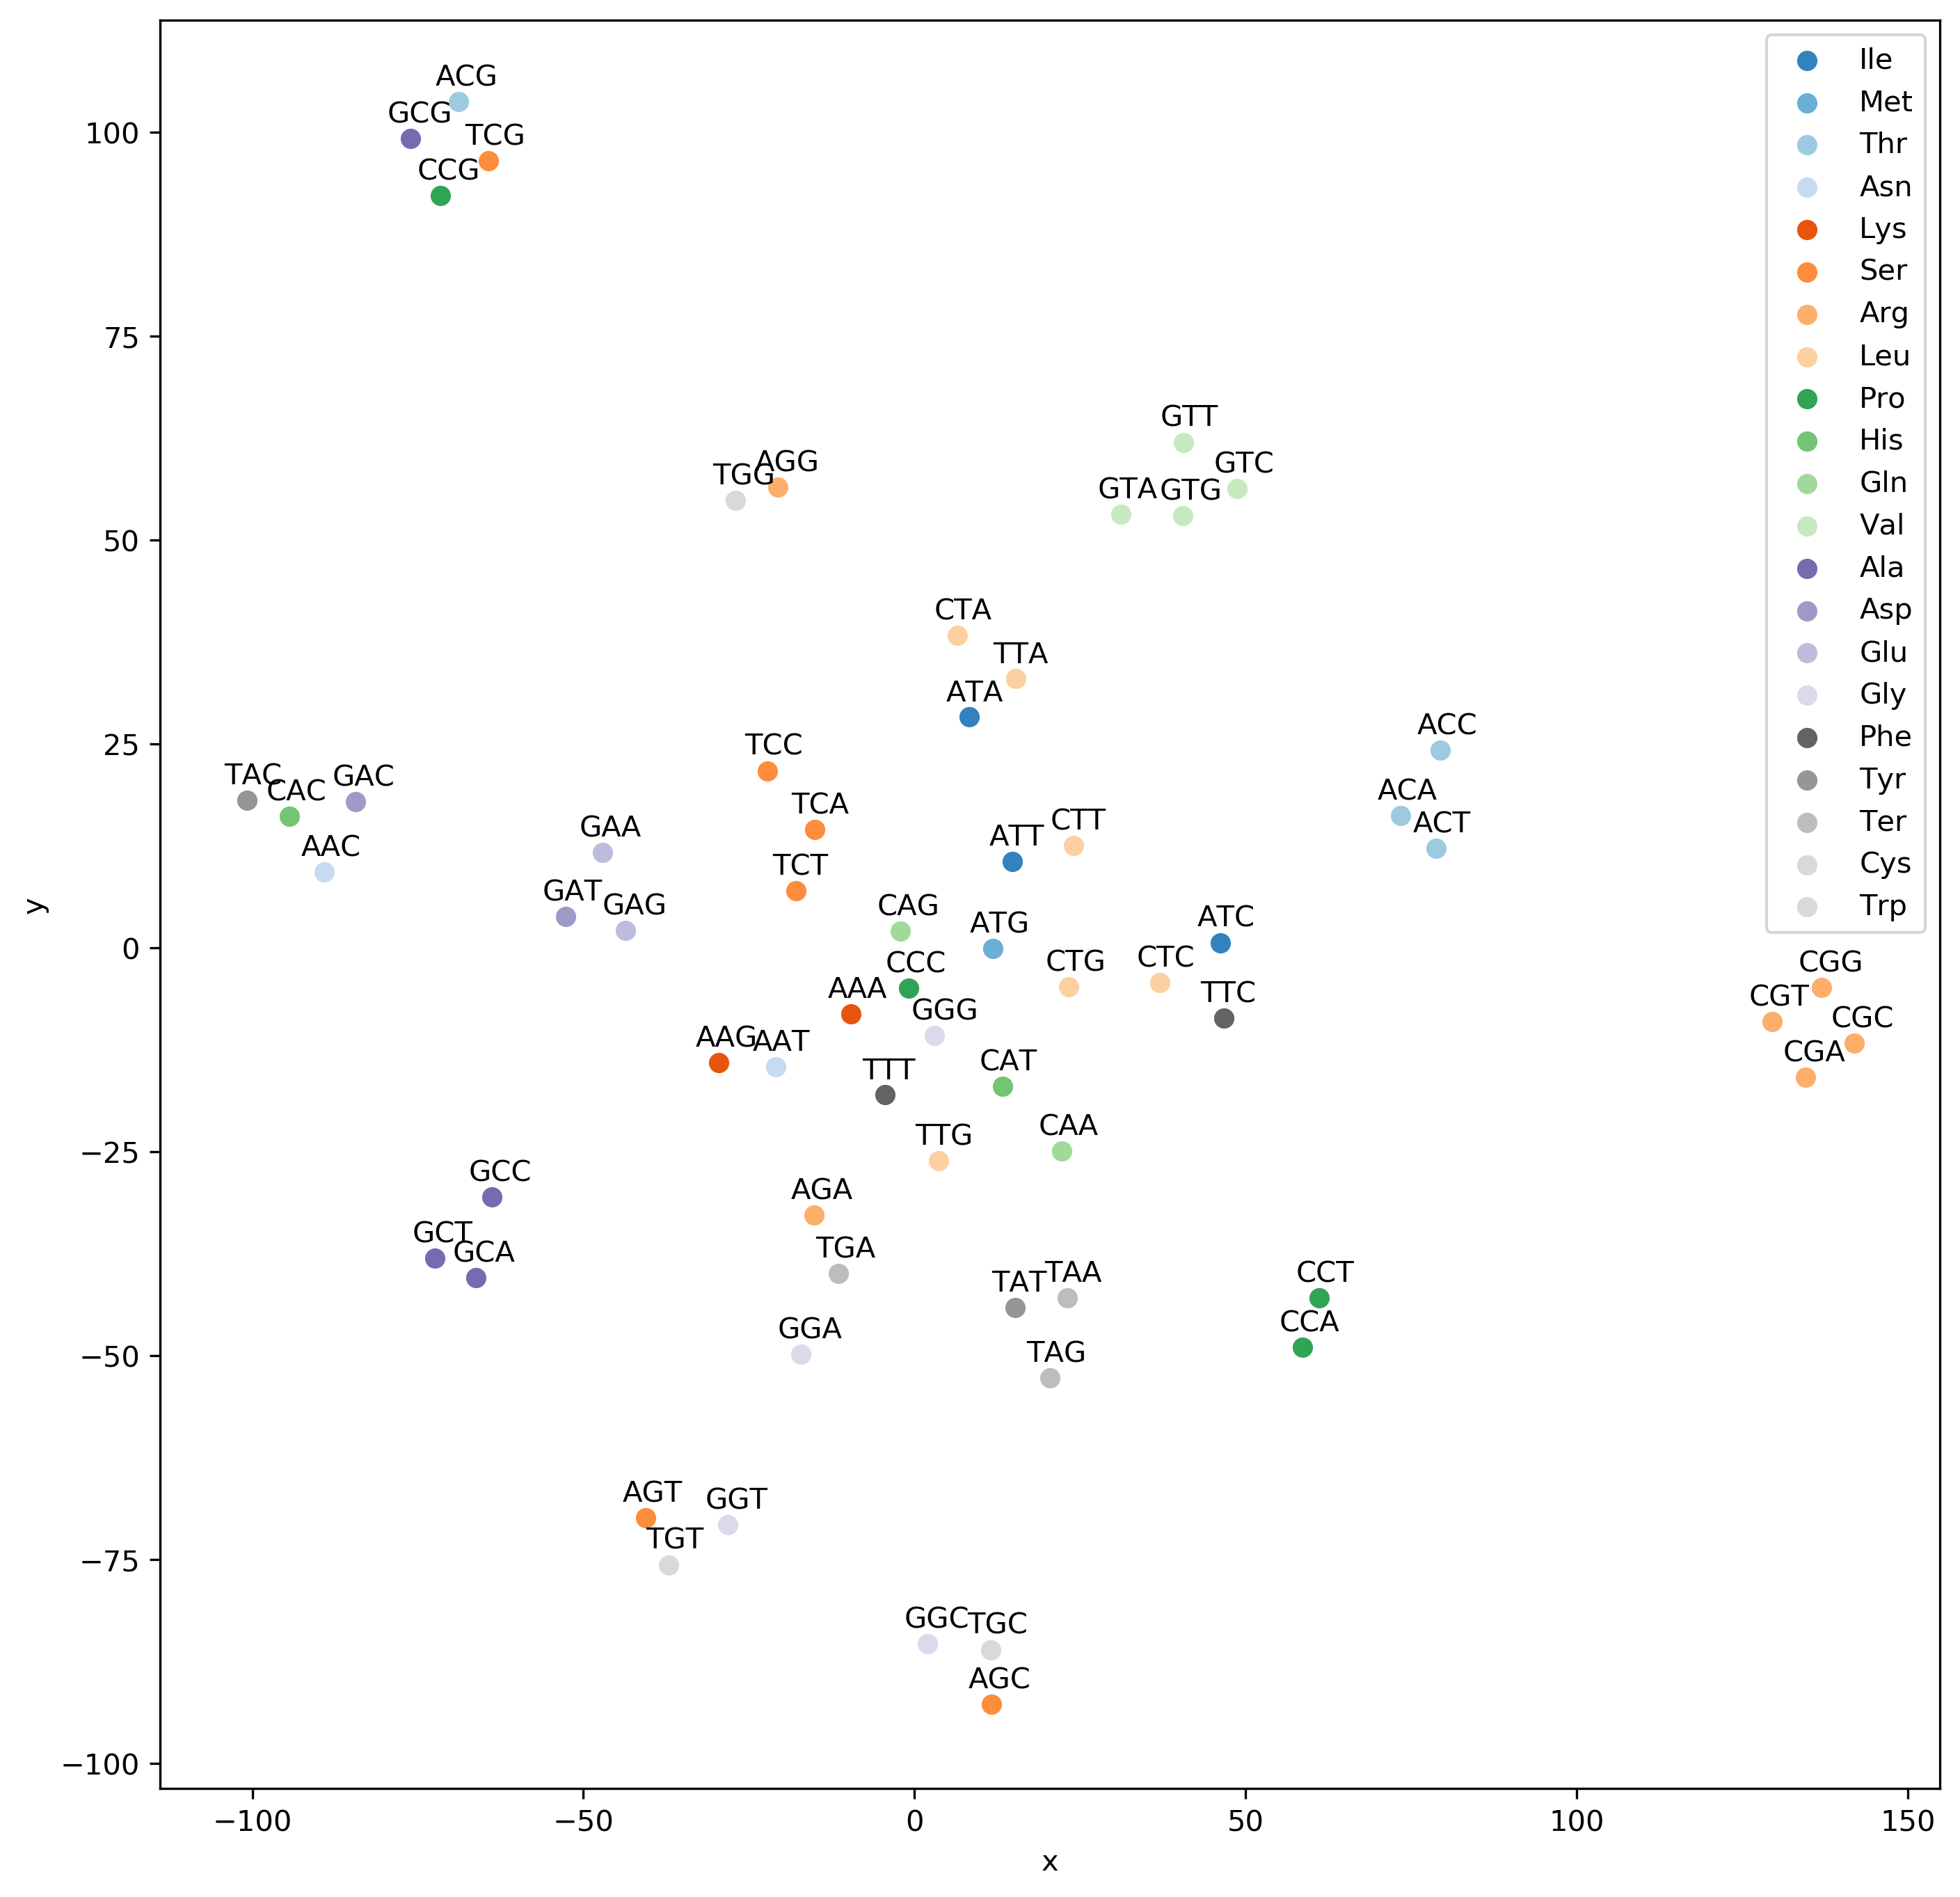
\includegraphics[width=1\textwidth]{../visualizations/ch4-methods/tsne_d2v_embeddings.png} 	
	\caption{
		The 2-dimensional embeddings obtained by applying t-SNE to the 100-dimensional learned representations of all 64 possible 3-mers. The corresponding amino acids are color-coded. 
	}
	\label{fig:tsne}
\end{figure}

We visualize the embeddings for all 64 possible 3-mers using Stochastic Neighbor Embedding (t-SNE) \cite{tsne} in Figure \ref{fig:tsne}.

Doc2Vec is trained to map words (3-mers) which occur in a similar context to similar representations. We observe that this often translates to mapping the same amino acids to similar representations. There are some instances when different amino acids are mapped together like the quartet Alanine (Ala), Threonine (Thr), Proline (Pro) and Serine (Ser) in the top-left corner. Why are exactly these different amino acids mapped together? The associated 3-mers reveal that these different amino acids share two nucleotides at the same position. This probably leads to these amino acids appearing in similar contexts.
%Displaying the 3-mers associated with the amino acids shows that this likely occurs because these different amino acids share two out of three nucleotides at the same positions. 
Overall, we take these visualizations as an indication that Doc2Vec was able to learn biologically useful embeddings for the overlapping 3-mers.
%[maybe] Making use of these pre-trained embeddings, each 140 nucleotide input sequence is split into overlapping 3-mers and mapped to a 100-dimensional vector. Like in the other models, a shallow MLP using these sequence features in conjunction with length features for classification.
\subsubsection{Putting it all together} \label{subsubsec:d2vinference}

\begin{figure}
	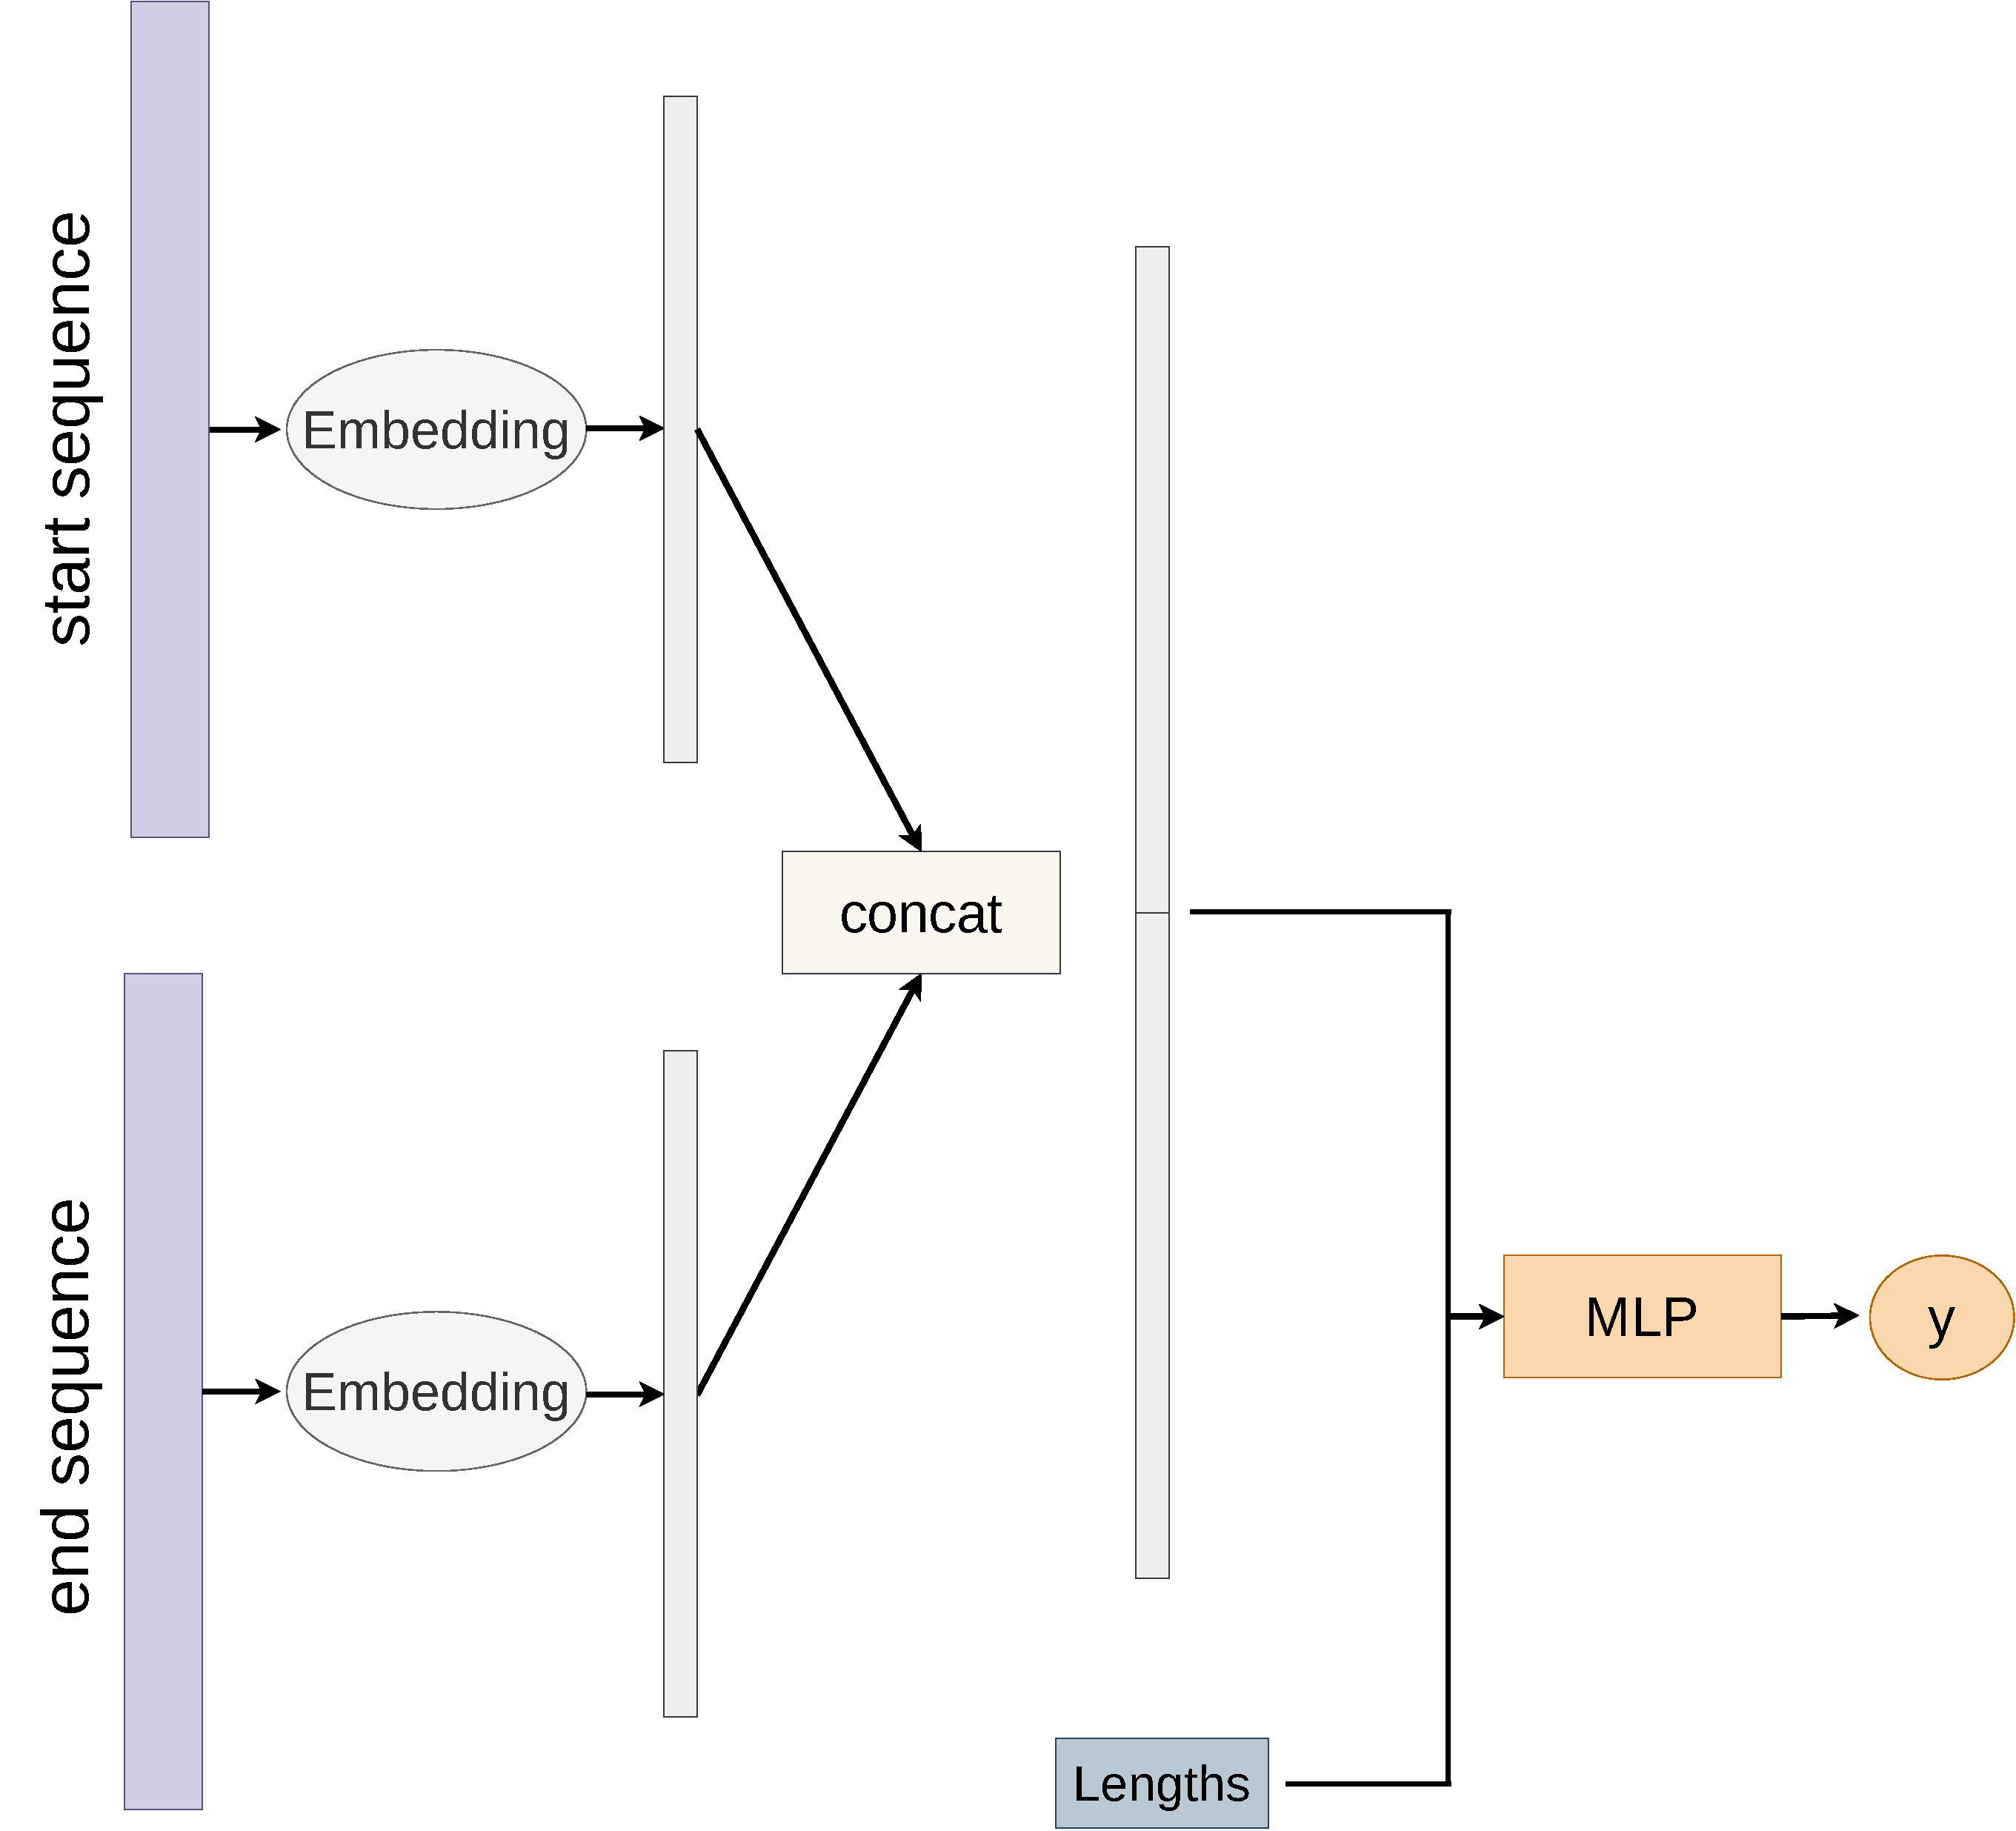
\includegraphics[width=0.7\textwidth]{../visualizations/ch4-methods/d2v.pdf} 	
	\caption{
		Architecture of D2V. 
	}
	\label{fig:d2v_arch}
\end{figure}

The resulting model uses the pre-trained Doc2Vec network to obtain a 100-dimensional embedding of the extracted nucleotide sequences around the exon start and exon end. These two embeddings, along with the length features, are then concatenated and given to a shallow MLP to obtain the final prediction. We refer to this model as Doc2Vec (D2V) and visualize it in Figure \ref{fig:d2v_arch}. 



%During inference, the Doc2Vec model outputs 100-dimensional embeddings for each input sequence. These, along with the length features, are fed into the shallow MLP for classification. The shallow MLP consists of two layers with 16 and 8 neurons each respectively followed by a dropout layer with dropout probability of 0.2.


%[discussion of the tsne embeddings here]
%research on what to write:
%Doc2Vec will map words (3-mers) which are used in similar contexts to similar representations
%wil: codon usage bias; not all encodings of a codon will be used with the same frequency
%the bias of codon usage at exon boundaries
%Laurence Hurst paper looks at biases in the first and last 30 nucleotides within an exon



\subsection{RASC: BiLSTM and Attention-based} \label{subsec:bilstm}

\subsubsection{Seq2Seq} \label{subsubsec:seq2seq}
Sequence-to-sequence learning (Seq2seq) \cite{seq2seq} is a general Deep Learning-based framework for mapping one sequence to another. The first part of the framework is an encoder which processes the input symbol-by-symbol and produces a vector representation for each input symbol. The second part is a decoder which predicts the output sequence symbol-by-symbol based on the representation computed by the decoder. In the first timestep, the decoder uses the last output of the encoder and in all other timesteps, it uses its own output from the previous time step as input. The encoder and decoder are typically RNN-based networks such as LSTMs \cite{lstm} or GRUs \cite{gru}. Encoder and decoder are jointly trained to maximize the probability of a correct output. This framework has been particularly successful in machine translation (MT): for instance, Google announced in 2016 that it started using them for their MT \cite{googlemt2016}. Figure \ref{fig:encdec} visualizes an encoder-decoder model.

\begin{figure}
	\centering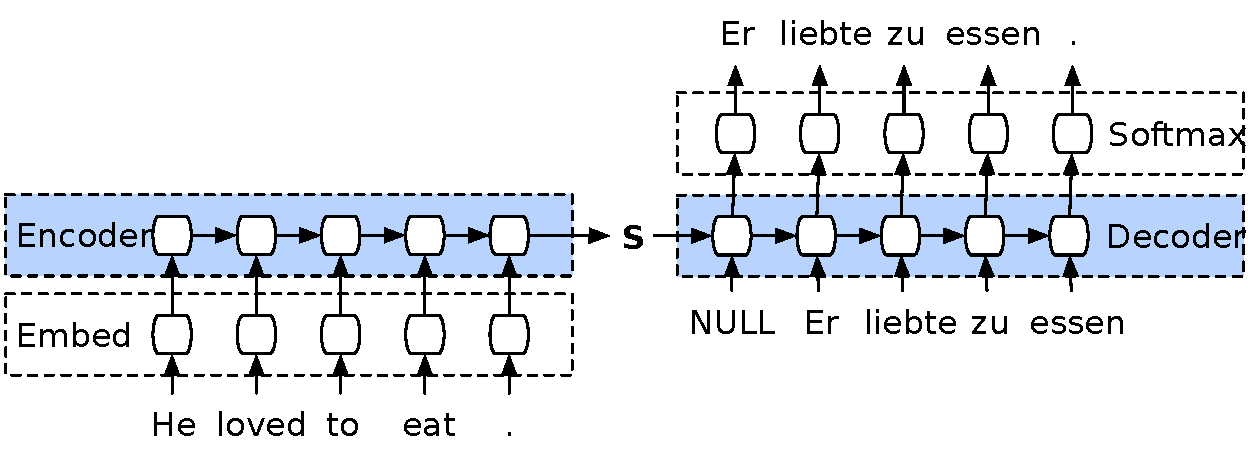
\includegraphics[width=0.9\textwidth]{../visualizations/ch4-methods/enc_dec.pdf} 
	\caption{An encoder-decoder model \cite{ruderencdecgraphic} translates the English sentence `He loved to eat' to the German sentence `Er liebte zu essen'. The decoder takes the last hidden cell state of the encoder as initial input and generates the output token-by-token. The decoder takes its own previous output as prompt for the next output and stops generating output token when it generates a `.'-token. }
	\label{fig:encdec}
\end{figure}

%Sutskever, I., Vinyals, O., & Le, Q. V. (2014). Sequence to sequence learning with neural networks. In Advances in Neural Information Processing Systems.
%https://smerity.com/articles/2016/google_nmt_arch.html
%https://ruder.io/a-review-of-the-recent-history-of-nlp/index.html#2013wordembeddings
\subsubsection{Are you paying attention?}
In the original Seq2seq framework, only the last state of the encoder is passed to the decoder. This means that the encoder needs to encode all the information observed in the input sequence into its last state. While theoretically possible, \cite{attention} hypothesized that this informational bottleneck hampers performance in practice. They proposed removing this bottleneck by introducing the attention mechanism. Attention is a mechanism whereby the decoder can access all the representation generated by the encoder at once and can `choose' to focus on (attend to) the most important ones. Introducing attention lead to large performance gains across Seq2seq-based models and quickly became standard practice \cite{attentionforms}. \\
The attention mechanism also adds interpretability to the model because it indicates which parts of the input sequence are most crucial for the model's prediction. Figure \ref{fig:attention_heatmap} visualizes what parts of an input sequence a model is paying attention to during an MT task. Attention is one of the most important innovations in Deep Learning research in recent years. It can theoretically be useful for any task where a model needs to make a decision based on certain parts of an input. For instance, the current state-of-the-art Transformer models \cite{allyouneed} \cite{bert} \cite{gpt3} forego recurrent networks completely and solely use attention within the encoder and decoder components. It has also been successfully used in other domains such as recommender systems \cite{attention_recommender_systems} or speech recognition \cite{attention_speech_recognition}. 


%However, as justified earlier, we won't focus on these models due to issues of scaling and the sufficiency of shallow networks for genomic prediction tasks.

\begin{figure}
	\centering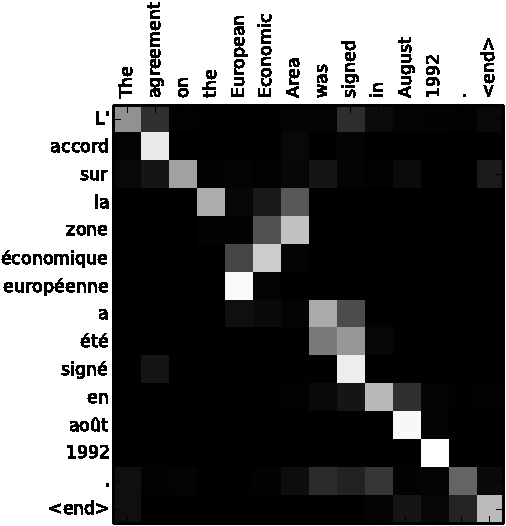
\includegraphics[width=0.7\textwidth]{../visualizations/ch4-methods/attention_heatmap.png} 
	\caption{Attention heatmap when translating a sentence from French to English. A brighter color indicates that the model pays more attention to a particular word. The order of the constituent words in `zone \'economique europ\'een' and `European Economic Area' is different between French and English, but the model learned to pay attention to the semantically corresponding word during translation. }
	\label{fig:attention_heatmap}
\end{figure}

%Bahdanau, D., Cho, K., & Bengio, Y. (2015). Neural Machine Translation by Jointly Learning to Align and Translate. In ICLR 2015.
%could also use graphics from this
%another attention reference: https://arxiv.org/pdf/1508.04025.pdf
%https://3.bp.blogspot.com/-3Pbj_dvt0Vo/V-qe-Nl6P5I/AAAAAAAABQc/z0_6WtVWtvARtMk0i9_AtLeyyGyV6AI4wCLcB/s1600/nmt-model-fast.gif
%alternative: https://machinetalk.org/2019/03/29/neural-machine-translation-with-attention-mechanism/
%Attention is a very general mechanism not limited to the Seq2seq framework and different forms of it (such as additive \cite{attention} or multiplicative attention \cite{allyouneed}) are used in practice. 


% how attention hasn't been used in genomics so far
%[transformer here and why I don't use it]
%[More applications of attention]
%It has been applied to constituency parsing (Vinyals et al., 2015)
%, reading comprehension (Hermann et al., 2015)
%, and one-shot learning (Vinyals et al., 2016)
%, among many others. The input does not even need to be a sequence but can consist of other representations as in the case of image captioning (Xu et al., 2015)
%, which can be seen in Figure 12 below
%\subsubsection{Integrating attention}
%Despite these successes, not many attention-based models have been applied to genomic data yet and in particular, none have been applied to the prediction of splicing behaviour. 
%Taking inspiration from the successful application and improved interpretability of the Seq2seq framework with attention in other domains, we also adopt it for constitutive exon classification. We now describe the modifications we made to the Seq2Seq and attention set-up known from MT for alternative splicing classification. In particular, we describe the attention mechanism in more detail as necessary for our second modification.

Despite these successes, not many attention-based models have been applied to genomic data yet and in particular, none have been applied to the prediction of splicing behaviour. 

\subsubsection{Why LSTM-based models were chosen over Transformers} \label{lstmvstransformer}
Perhaps surprisingly, we chose to not base our model on the Transformer network architecture:

In contrast to LSTMs who need to process all symbols in their input sequentially, Transformers can process them concurrently. This is the main advantage of Transformers over LSTMs and enables them to scale to enormous datasets and hundreds of millions (or billions \cite{gpt3}) of parameters \cite{allyouneed}.

However, we have no huge datasets to scale to: our largest exon dataset contains roughly 50,000 training samples and this already includes all the known cassette exon in the human genome. Creative use of data augmentation might increase dataset size by two or three factors, but even 150,000 training samples is still far smaller than the millions of training samples used in NLP. Scaling down Transformers models would mean they lose their main advantage over LSTMs: on small NLP datasets LSTMs and small (not-distilled \cite{distilbert}) Transformers perform similarly \cite{mogrifier}\cite{smalltransformerwin} and there is no clear consensus which approach is superior. 

%LSTM win: https://arxiv.org/abs/1909.01792
%Transformer win: https://arxiv.org/abs/1912.09713
Additionally, the autoregressive bias inherent to LSTMs aligns well with our knowledge about the biological reality: the spliceosome also processes information in the sequences piecewise. Opposed to LSTMs and the spliceosome, Transformers process their complete input concurrently.
%Transformers are stateless 
%and only add information about the relative positions of the input through the use of positional encodings. This would mean that the learning task of the Transformers is harder. bullshit because the same argument for language really


Thus, we base the encoder part of our model on the simpler LSTMs. 

\subsubsection{Modifying Seq2Seq}
We now describe the modifications we made to the Seq2Seq and attention set-up known from MT for alternative splicing classification and regression. In particular, we describe the attention mechanism in more detail as necessary for our second modification.



\subsubsection{Modification 1: MLP instead of a recurrent decoder}
As the name implies, models based on the Seq2seq framework take a sequence as input and give a sequence as output. This is achieved via using a recurrent decoder which outputs symbols until it outputs an <EOS> (end-of-sequence, e.g. a `.') token.
However, we only expect a single output: a scalar signifying the classification or frequency of the alternative splicing behaviour of an exon or junction. 
% However, in our case, the output will always be a single scalar. Thus, we don't require a recurrent decoder and instead use a shallow MLP in its place.
\subsubsection{Modification 2: Attention with a learned query vector}
The most common form of attention (multiplicative or dot-product self-attention \cite{allyouneed}), makes uses of conceptual queries and key-value pairs. A query, key and value matrix is assigned to each symbol in the input sequence. A given query is compared to all keys by computing a similarity score between the query and each key via the dot-product. The similarity scores are normalized through the use of a softmax layer. The normalized similarity scores are also commonly called the attention weights; keys similar to the query are weighted more. The output of the attention layer for a given query and input sequence is then the weighted vector sum obtained by multiplying each value by the attention weight of its respective key.
Putting the above intuition into formulas, the (dot-product self-) attention mechanism can be described more formally:

Initially, the query, key and value matrices $Q$, $K$ and $V$ are computed by multiplying the input with the query, key and value parameter matrices $W^Q$, $W^K$ and $W^V$:
$$Q, K, V = IW^Q, IW^K, IW^V$$
where $I \in \mathbb{R}^{l \times in}$, and $W^Q,W^K, W^V \in \mathbb{R}^{in \times out}$,
and $Q,K, V \in \mathbb{R}^{l \times out}$. $in$ corresponds to the number of features of each element in the input sequence to the attention layer, $out$ corresponds to the number of features in the output of the attention layer. $l$ corresponds to the number of elements in the input sequence.

Attention can be then computed as:
$$Z = attention(I) = softmax(QK^T)V$$
where $Z \in \mathbb{R}^{l \times out}$. 
Note that this makes use of the fact that $Q\cdotp K = QK^T$ where $\cdotp$ denotes the dot product.
%This form of attention is also visualized in Figure !](https://jalammar.github.io/images/t/self-attention-matrix-calculation.png) and ![
%from https://jalammar.github.io/illustrated-transformer/
%remove this division by square-root -- maybe ask Kuba how to photoshop this away


As shown, multiplicative self-attention computes a separate query for each input token. It is called self-attention because it allows a sequence to pay attention to `itself'. (Unmasked) self-attention is mainly used in the encoder part of Transformer architectures to improve the representation for each word.\\
However, our objective in using attention is not to improve the representation for each symbol in a sequence (finding a good representation is the task of the encoder), but to select the most important features from an input sequence. The conceptual query for our task is also always the same independent of input: is this exon constitutively spliced or not?
%thought: this also naturally happens in seq2seq models when they use attention -- how is what I am doing differently?
Thus, we adapt the attention mechanism so that we learn a single, input-independent query ${Q}^* \in \mathcal{R}^{1 \times out}$. The output of the attention layer is now computed as:
$$Z^* = {attention}^*(I) = softmax({Q}^*K^T)V$$

%decided against explaining innovation as two-points with (1) one query and (2) independent of input because I felt unsure of (2)

where $Z^* \in \mathbb{R}^{1 \times out}$. Note that the query matrix ${Q}^*$ is directly learned in the attention block and not multiplied with the input, giving rise to its input independence. The output $Z$ is now a weighted sum of the nucleotide representation in the input sequences which the model deemed most crucial to pay attention to.
The input $I$ is a concatenation (along the first dimension) of the representations given by the encoder for the nucleotide sequence around the exon start and exon end.



\subsection{Further modifications of the attention mechanism} \label{subsec:alternative_attention}
In the following, we introduce three further modifications of the attention mechanism which we evaluated separately from the modifications described so far.
%In the following, we introduce multiple extensions which were attempted which didn't lead to improved results. For most of these, initial results clearly showed that the results weren't improved by using them. As such, we didn't test these extensions more extensively than initial experiments because we felt the initial results were already instructive enough and no further investigation was warranted. Thus, the analysis of the results won't be as extensive as for the extensions which worked.



\subsubsection{No query matrix} \label{subsubsec:noquery}
As the query matrix ${Q}^*$ is the same independent of the exact input sequences, it could be possible to remove the query matrix and compute the attention weights sorely based on the key matrix $K$.
This is possible by learning a key weight matrix $W^{K_{no\_query}} \in \mathcal{R}^{in \times 1}$ and computing attention as:
$$K_{no\_query} = IW^{K_{no\_query}}$$
$$Z_{no\_query} = {attention}^{**}(I) = softmax(K^*)V$$
where $K_{no\_query} \in \mathbb{R}^{l \times 1}$ and $Z_{no\_query} \in \mathbb{R}^{1 \times out}$. This has the advantage of reducing the number of learnable weights as adapted the key weight matrix $W^{K_{no\_query}} \in \mathcal{R}^{in \times 1}$ is smaller than the initial key weight matrix $W^{K} \in \mathcal{R}^{in \times l}$.  


\subsubsection{Multiple attention heads} \label{subsubsec:heads}
Having one set of query, key and value matrices limits the model to one representational subspace (one way of `interpreting' the input). It might be useful for the model to have multiple representational subspaces. This is usually achieved \cite{allyouneed} via $h$ different sets of query, key and weight matrices $W^{Q^*_1}, W^{K_1}, W^{V_1}, \dots W^{Q^*_{h}}, W^{K_{h}},W^{V_{h}}$ producing $h$  outputs $Z_1, \dots, Z_{h}$. Applying this extension in our context engenders the following formulas:
$$K_i, V_i = IW^K_i, IW^V_i$$
$$Z^*_i = {attention}^*_i(I) = softmax({Q}^*_iK^T_i)V_i$$
Note that the query weight matrices $W^{Q^*_1}, \dots, W^{Q^*_h}$ are again directly learned, like in the single head case. 

The final output matrix $Z_{final} \in \mathcal{R}^{l \times out}$ is then computed as:
$$Z_{final} = concat(Z_1^*, \dots, Z_{h}^*) W^O$$
where the concatenation occurs along the second dimension and $W^O \in \mathcal{R}^{out * h \times out_{new}}$. $out_{new}$ represents the new output dimension of the attention layer, which is arrived at by combining the dimensions of the $h$ attention heads.

While these extra representational subspaces might make the model more powerful and also more robust (in the sense that multiple attention heads act like an ensemble model), it also increases the number of learnable weights potentially leading to overfitting.
\subsubsection{Convolution in attention heads} \label{subsubsec:attention_conv}
The information contained in a single nucleotide is very low. 
This motivated \cite{ghentransformers} to integrate an additional 1D convolution into the computation of the query, key and value matrices Q, K and V which is applied after the multiplication with the weight matrices $W^Q, W^K$ and $W^V$. This convolution allows the model to more effectively integrate information from multiple neighbouring nucleotides. This extension can also be understood as an alternative to splitting the input nucleotide sequence into k-mers (similar to the split into overlapping 3-mers for the input of the D2V model \ref{subsubsec:kmers}) and provided better results than splitting the input nucleotide sequence into k-mers when using a Transformer network for a genome annotation task in \cite{ghentransformers}.
In formulas, we can describe the adapted attention mechanism as:
%Keeping in mind the modification of directly learning the query matrix, this leads to:
$$K_{conv}, V_{conv} = conv(K), conv(V)$$
$$Z^*_{conv} = {attention}_{conv}^*(I) = softmax({Q}^*K_{conv}^T)V_{conv}$$
where $K$ and $V$ are both fed through the same convolutional layer to arrive at $K_{conv}$ and $V_{conv}$. The weight matrix corresponding to the convolutional layer is chosen so it has the same number of feature dimensions as $K$ and $V$, that is, $W_conv \in \mathbb{R}^{out \times kernel \times out}$. $kernel$ denotes the size of the convolutional kernel. 
The padding is chosen so that the first dimension of $K$ and $V$ stays the same which leads to $K_{conv}, V_{conv} \in \mathbb{R}^{l \times out}$.
%The number of convolutional filters and the padding are chosen so that the dimensions of the $K$ and $V$ matrices don't change, that is, $K_{conv}, V_{conv} \in \mathbb{R}^{l \times out}$.

To incorporate the domain knowledge that the input sequences to our model come from two different places in the genome, the convolution is applied in such a way that it does not mix the information between the sequences around the exon start and around the exon end. To achieve this, we implemented the following computations:
$$K^{start}, K^{end} = I^{start}W^K, I^{end}W^K,$$
$$K^{start}_{conv}, K^{end}_{conv} = conv(K^{start}), conv(K^{end})$$
$$K_{conv} = concat(K^{start}_{conv}, K^{end}_{conv})$$
where the $start$ and $end$ superscript respectively refer to the sequence around the start and end of the exon. The concatenation is along the first dimension (so the length of the sequences). The analogue computation was implemented for $V_{conv}$.


A small implementational detail regarding the attention blocks: the query, key and value parameter matrices are implemented via a linear layer with the appropriate dimensions. These also learn bias weights which are added to the output by default. While in theory the bias weights should be turned off to implement exactly the shown formulas, in practice other attention mechanism implementations leave these turned on \cite{annotatedtransformer} and so we follow suit. Thus, to be precise, the query, key and value matrix computation should be:
$$K, V = IW^K + B^K, IW^V + B^V$$
$$Z^* = {attention}^*(I) = softmax(({Q}^*K^T)+B^{Q^*})V$$
where the query, key and value bias matrices $B^{Q^*}, B^K$ and $B^V \in \mathbb{R}^{1 \times out}$.

\subsubsection{Putting it all together:} 
Like in a Seq2Seq model, an RNN-based Encoder is used to capture a representation of the input sequence. We attend to the most important representations of the encoded input using the modified attention mechanism we introduced. The resulting feature vector is concatenated with the lengths and given to a shallow MLP. 
%selecte Instead of a recursive decoder, we use a shallow MLP in its place. 

The input to the encoder blocks is a dense 4-dimensional embedding of the one-hot encoded sequences. This dense embedding is the same for each sequence and jointly learned during training. The extra embedding layer is included as previous work \cite{embeddingneeded} has shown that otherwise, the model might suffer from limited generalization performance, caused by the sparsity of the one-hot encoded representations. 

LSTM cells opposed to unmodified RNNs are used as encoder as LSTMs have been shown to be better at retaining information over long sequences and avoiding the vanishing and exploding gradient problems \cite{lstm}. In particular, we use Bidirectional LSTM (BiLSTM) \cite{bidirection} to model that the splicing of an exon likely depends on bi-directionally interacting factors. A separate BiLSTM is used for finding for encoding the exon start and exon end sequence. 

As this lead to empirically better results, we also introduce a 1D batch normalization layer \cite{batchnormalization} before the attention layer. A dropout layer in the attention head is used for the same reason. 

We pre-empt the results chapter by noting that we only use the extension of multiple attention heads of the three additional modifications of the attention mechanisms we considered. 
The architecture of our model is visualized in Figure \ref{fig:attnbilstm}. We refer to this new model as Recursive Attentive Splicing Code (RASC). In the experiments section, we validate the choice of introducing the attention mechanism to RASC, by removing it and evaluating the model which only uses the hidden state of the BiLSTMs. We denote this model as Recursive Splicing Code (RSC).
\begin{figure}
	\centering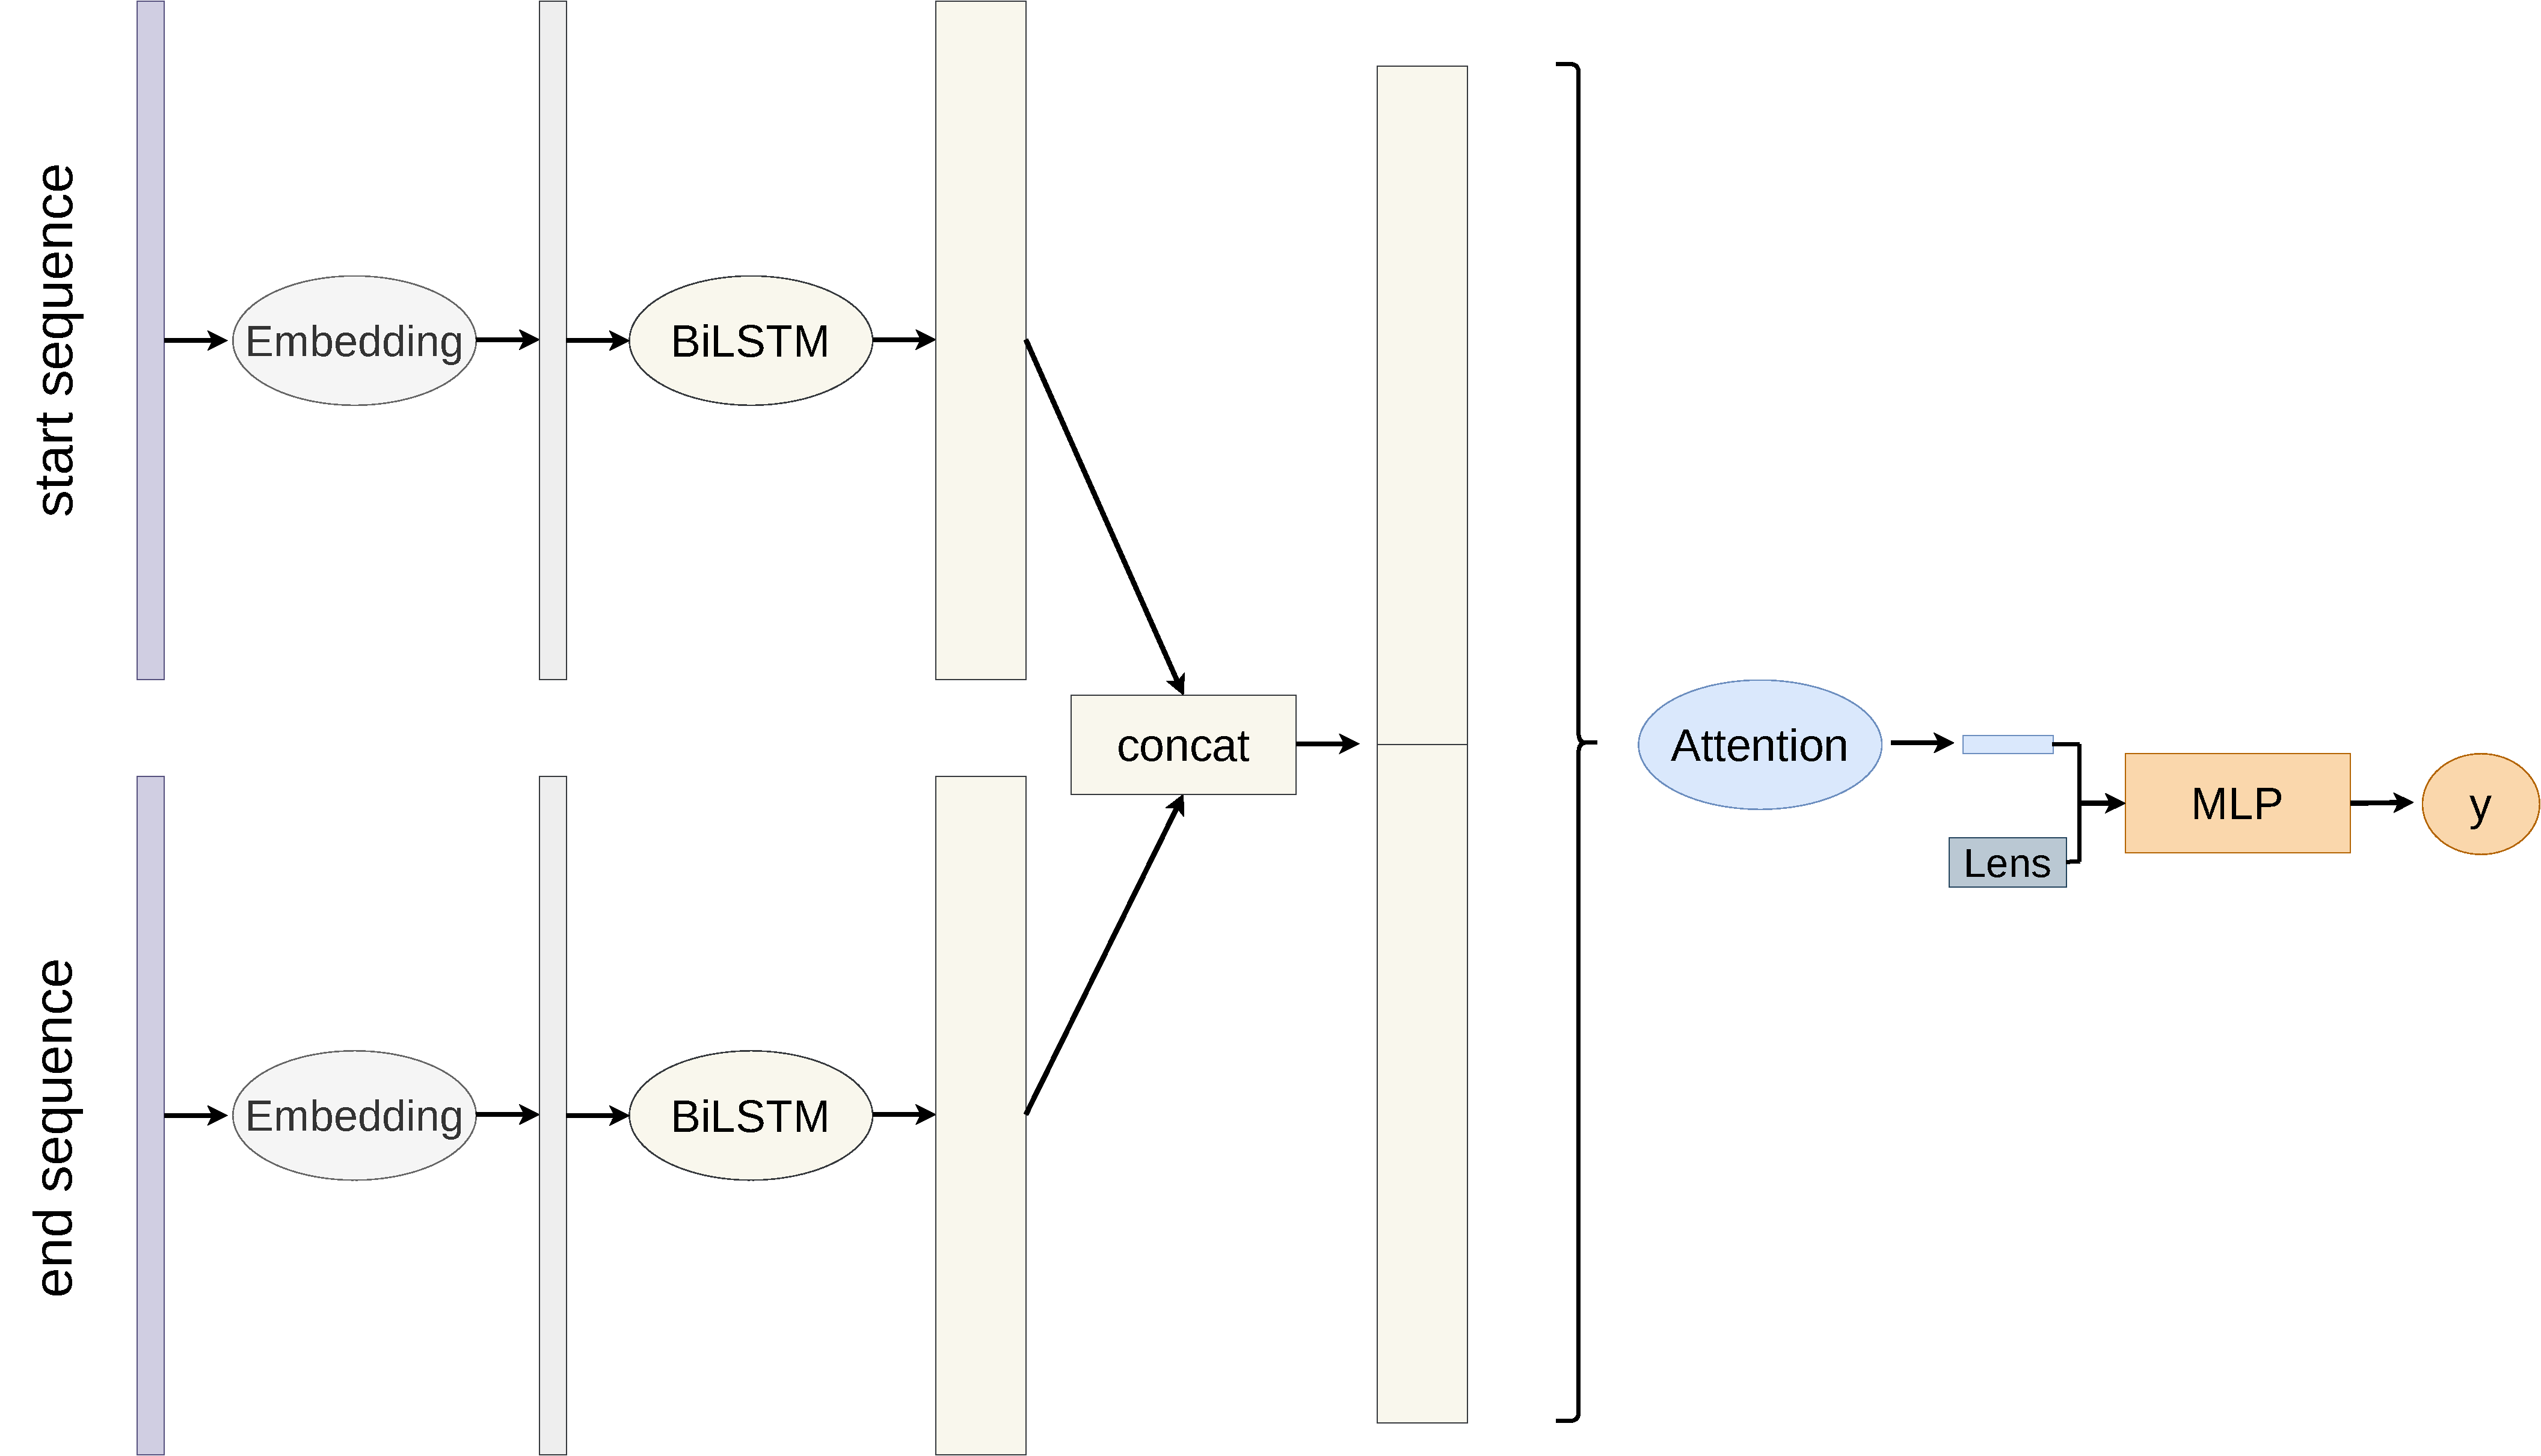
\includegraphics[width=1\textwidth]{../visualizations/ch4-methods/visualizations-AttnBiLSTM.pdf} 
	\caption{Architecture of RASC. }
	\label{fig:attnbilstm}
\end{figure}


%   old motivation:
%The architecture of this model can be motivated in two ways:
%1) Similar to DSC, we use two blocks for feature extraction. However, incorporating the knowledge that our input data is a sequence, we use an RNN for this feature extraction. In particular, under the assumption that bidirectional context is important for this task, we use bidirectional LSTM (BiLSTM). Like DSC, a shallow MLP uses the obtained features of both blocks for classification.
%2)
%The final model is very similar to the current state-of-the-art splicing code for predicting the inclusion rate of a cassette exon [distributed], as introduced in [related works].
%maybe: (could make my motivation seem shallow)
%This is a standard LSTM architecture and a similar architecture have been successfully applied to the related task of finding new splice junctions. [https://arxiv.org/pdf/1512.05135.pdf, https://www.sciencedirect.com/science/article/pii/S0010482519304135]
%simple feature extraction + classification model as eg in [https://www.researchgate.net/figure/An-example-of-bidirectional-LSTM-tagger-architecture_fig1_330276457 ] -- 5 citations

For RASC, the hyperparameter space was a lot larger and model performance was very sensitive to the hyperparameter choice. The most crucial hyperparameters were the number of encoder dimensions and the number of dimensions of the attention layer. Hyperparameters were optimized via a grid search on the HipSci MAJIQ dataset.


\section{Implementation, training and evaluation} \label{sec:implementation_details}
\subsection{Implementation} \label{subsec:implementation_details}
All models, except the Doc2Vec network, were implemented using the PyTorch library (version 1.5.0) \cite{pytorch}. The Doc2Vec model was implemented using the gensim library (version 3.8.3) \cite{gensim}. PyTorch and gensim are both standard choices when implementing Deep Learning algorithms or text embedding models. The data processing was done using a mixture of Python and Bash scripts as well as the software tools MAJIQ and SUPPA described in section \ref{subsubsec:majiq} and \ref{subsubsec:suppa}. The latest versions of SUPPA (version 2.3) and MAJIQ (version 2.0) available as of July 2020 were used. The complexity induced by the use of a large number of different datasets and data processing methods was handled by standardizing the shape of the final training samples. Even though 10 different datasets and 3 different models are used, the codebase contains only 2 different data loader and trainer classes.
%they all use the same data loading and training code. %

The structure of the repository was based on the PyTorch Deep Learning Project template available at \url{github.com/victoresque/pytorch-template}. This template provides abstract classes for data loaders, trainers and the models themselves. These abstract classes already contain a lot of the implementation-independent code to log results and train and save models. These base classes were then extended with implementation-specific code as e.g. exact data formats. Using this structure avoids the duplication of a lot of boilerplate code.\\
To run an experiment, the experimental settings are defined in a separate JSON file. This allows for easy and unambiguous reproduction of results. All experiments for whom results in this study are shown are available as JSON files that define the exact parameters used.
The code repository itself contains multiple README which give more details about the code structure, how to run experiments and what naming conventions are used. 
%which go into more details towards the structuring and using of the code and also define naming conventions.\\

%total codebase contained roughly ... lines of code. the majority of these were in preprocessing section [maybe exclude this]

\subsection{Training} \label{subsec:training_details}
The training was done using one NVIDIA GeForce GTX 1080 Ti GPU. This proved to be sufficient as initial exploratory experiments showed no advantage of using deep networks and the networks we evaluate are all relatively shallow. For training and testing, we randomly split each dataset into 10 folds; in a given run, 8 folds were used for training, 1 fold for validation and 1 fold for testing. Each model was trained with different folds 9 times and we compute the mean test set performance.\\
%The median training times for one complete training run were 1-5 minutes 
The models were trained with early stopping on the validation fold until they stopped improving for 15 epochs. This typically occurred after 70 - 150 training epochs.

The pre-training of the Doc2Vec model on the human genome took 3 hours. 

DSC, D2V and RASC respectively contain 20,001, 6,801, and 66,861 trainable weights. In absolute terms, all of these models are still small compared to models known from Computer Vision and Natural Language Processing. The number of training weights is also reflected in the training times with the models respectively taking between 5 to 30 minutes, 1 to 5 minutes and 15 to 75 minutes to train once (depending on dataset). The increased training time of RASC is likely also influenced by LSTMs processing the input sequentially.

%An advantage of convolutional neural networks is that they are more parallelizable than RNNs, as the state at every timestep only depends on the local context (via the convolution operation) rather than all past states as in the RNN.
The hyperparameters used for training the models are given in Table \ref{table:hyperparameters}. More details on the Doc2Vec pre-training procedure and hyperparameters values are given in Section \ref{app:d2v} in the appendix.

\subsubsection{Loss}  \label{subsubsec:loss}
All models were trained to minimize the binary cross-entropy loss:
$$\mathbb{L} = - (y \log(\hat{y}) + (1 - y) \log (1 - \hat{y}))$$
where the ground truth $y \in \{0, 1\}$ and the prediction of the model $\hat{y} \in [0, 1]$. The binary cross-entropy loss is the standard loss for training Deep Learning-based (binary) classifiers.

\subsection{Evaluation}

To evaluate the models, we report the mean test set performance and standard deviation across (cross-validation) runs. 
Where we established in a base experiment that the variance for a given model was low between runs (lower than $\sim$1\%), we only trained the model once in follow-up experiments for practical reasons.

Previous studies have shown that model performance varies significantly between lowly and highly included alternatively spliced exons \cite{dsc} \cite{buschhertel}. Thus, following previous work, we split our test set into a set of highly (PSI > 80\%) and a set of lowly to moderately included, alternatively spliced exons (PSI <=80\%). Both sets contain all constitutive exons. We denote the first set as high PSI dataset (HighPSI), the second as low PSI dataset (LowPSI) and the complete test as all PSI dataset (AllPSI). We evaluate our models on all three datasets.


\subsubsection{Metrics} \label{subsubsec:metrics}
As in previous work \cite{dsc} \cite{buschhertel}, we use the Area under the receiver operating characteristic curve (AUC) as the primary evaluation metric. The AUC provides an aggregate measure of the classification performance across all possible decision thresholds.\\
However, the AUC doesn't provide information about model performance at a particular decision threshold. To evaluate whether a model is fit for clinical use, decision threshold-specific metrics like sensitivity and specificity are crucial to know.
To evaluate these, we analytically compute the decision threshold which maximizes the F1 score. The F1 score provides an aggregate measure which treats precision and recall equally and is defined as the harmonic mean of precision and recall. It is a common measure to evaluate the performance of classifiers and we use it as a starting point for our further analysis. 

Again following previous work \cite{d2vsplicing} \cite{jha}, we use the explained variance $R^2$ to evaluate model performance on the regression task. 
%To evaluate these, a decision threshold above which all outputs are counted as positive and below which all outputs are counted as negative. For our further analysis, we use the decision threshold which maximizes the F1 score and also evaluate the sensitivity and specificity. 

%For our analysis, we analytically compute and use the decision threshold which maximizes the harmonic mean of the precision and recall, that is, the F1 score. 

% : say which metrics you actually evaluate here
%Naively, this threshold may be set to 0.5, but this will not necessarily be the 'optimal' decision threshold in the sense of the optimality we define.  that it doesn't balance the trade-off between false positive false negatives in the way we want. We analytically compute the decision 
%
%For further analysis, we also evaluate sensitivity, specificity and F1 score on the HipSci MAJIQ dataset. Since the AUC is an aggreg
%
%The AUC implicitly treats sensitivity and specificity as equal when averaged across all thresholds. 
%On the unbalanced datasets, we also evaluate recall, specificity and the F1 score since the AUC does not give information about the . 
%However, some of our datasets were unbalanced. This may lead to a degenerating behaviour where a model only predicts the majority class. Additionally, only looking at the AUC does not give a good sense of the .... specificity.. recall?
%This is not captured by the AUC. \\
%Thus, we also evaluated the F1 of our models when working with an unbalanced dataset as in the case of the HipSci-based dataset processed with MAJIQ.
%The output of our models is a single, continuous scalar $\hat{y} \in [0, 1]$. As the AUC itself is an aggregate measure across all decision thresholds, we don't need to set it to a certain value that translates the continuous prediction into a discrete positive or negative class prediction. To compute the F1 score, we do. Naively, this threshold may be set to 0.5; that is, all outputs above 0.5 will be interpreted as a prediction of the positive class and all other outputs as a prediction of the negative class. However, this threshold may not be optimal to maximize the F1 score, especially when working with unbalanced datasets. We choose the threshold which maximizes the F1 score on the test set.


\begin{table}[h!]
	\centering
	\begin{tabular}{| l | c |} 
		\hline
		\textbf{DSC}\\
		\hline
		Kernel filters & 32, 8, 8 \\
		Kernel size & 7, 5, 3 \\
		Dropout (after fully-connected layer) & 0.5\\
		Neurons fully-connected layer & 64 \\
		Dropout (after convolution) & 0.2, 0.2, 0.2\\
		\hline
		\textbf{D2V}\\
		\hline
		Embedding dimension & 100\\
		Neurons (fully-connected layers) & 32, 8\\
		Dropout (fully-connected layers) & 0.2, 0.2\\
		\hline
		\textbf{RASC} \\
		\hline
		Dense embedding dimensions & 4\\
		BiLSTM dimension & 50\\
		BiLSTM layers & 1\\
		Attention heads & 4\\
		Attention head dimension & 50\\
		Dropout (attention head) & 0.4 \\
		Attention layer output dimension & 100\\
		Neurons fully-connected layer & 128\\
		Dropout (after fully-connected layer) & 0.5\\
		\hline
	\end{tabular}
	\caption{Hyperparameters of the three models
	}
	\label{table:hyperparameters}
\end{table}
